\documentclass[11pt]{aghdpl}
% \documentclass[en,11pt]{aghdpl}  % praca w języku angielskim

% Lista wszystkich języków stanowiących języki pozycji bibliograficznych użytych w pracy.
% (Zgodnie z zasadami tworzenia bibliografii każda pozycja powinna zostać utworzona zgodnie z zasadami języka, w którym dana publikacja została napisana.)
\usepackage[english,polish]{babel}

% Użyj polskiego łamania wyrazów (zamiast domyślnego angielskiego).
\usepackage{polski}

\usepackage[utf8]{inputenc}

% dodatkowe pakiety

\usepackage{mathtools}
\usepackage{amsfonts}
\usepackage{amsmath}
\usepackage{amsthm}

% --- < bibliografia > ---

\usepackage[
style=numeric,
sorting=none,
%
% Zastosuj styl wpisu bibliograficznego właściwy językowi publikacji.
language=autobib,
autolang=other,
% Zapisuj datę dostępu do strony WWW w formacie RRRR-MM-DD.
urldate=edtf,
% Nie dodawaj numerów stron, na których występuje cytowanie.
backref=false,
% Podawaj ISBN.
isbn=true,
% Nie podawaj URL-i, o ile nie jest to konieczne.
url=false,
%
% Ustawienia związane z polskimi normami dla bibliografii.
maxbibnames=3,
% Jeżeli używamy BibTeXa:
backend=bibtex,
seconds=true
]{biblatex}

\usepackage{csquotes}
% Ponieważ `csquotes` nie posiada polskiego stylu, można skorzystać z mocno zbliżonego stylu chorwackiego.
\DeclareQuoteAlias{croatian}{polish}

\begin{filecontents}{bibliografia.bib}
@online{Bonding,
  author = {Stu Borman},
  title = {Spying On Bond Making In Solution},
  date = {2015-02-19},
  url = {http://cen.acs.org/articles/93/i8/Spying-Bond-Making-Solution.html},
  urldate = {2015-03-03},
  addendum= {All about dicyanoaurate, has links to papers.}
}
\end{filecontents}

\addbibresource{bibliografia.bib}

% Nie wyświetlaj wybranych pól.
%\AtEveryBibitem{\clearfield{note}}


% ------------------------
% --- < listingi > ---

% Użyj czcionki kroju Courier.
\usepackage{courier}

\usepackage{listings}
\lstloadlanguages{TeX}

\lstset{
	literate={ą}{{\k{a}}}1
           {ć}{{\'c}}1
           {ę}{{\k{e}}}1
           {ó}{{\'o}}1
           {ń}{{\'n}}1
           {ł}{{\l{}}}1
           {ś}{{\'s}}1
           {ź}{{\'z}}1
           {ż}{{\.z}}1
           {Ą}{{\k{A}}}1
           {Ć}{{\'C}}1
           {Ę}{{\k{E}}}1
           {Ó}{{\'O}}1
           {Ń}{{\'N}}1
           {Ł}{{\L{}}}1
           {Ś}{{\'S}}1
           {Ź}{{\'Z}}1
           {Ż}{{\.Z}}1,
	basicstyle=\footnotesize\ttfamily,
}

% ------------------------

\AtBeginDocument{
	\renewcommand{\tablename}{Tabela}
	\renewcommand{\figurename}{Rys.}
}

% ------------------------
% --- < tabele > ---

\usepackage{array}
\usepackage{tabularx}
\usepackage{multirow}
\usepackage{booktabs}
\usepackage{makecell}
\usepackage[flushleft]{threeparttable}

% defines the X column to use m (\parbox[c]) instead of p (`parbox[t]`)
\newcolumntype{C}[1]{>{\hsize=#1\hsize\centering\arraybackslash}X}


%---------------------------------------------------------------------------

\author{Piotr Jaromin}
\shortauthor{P. Jaromin}

%\titlePL{Przygotowanie bardzo długiej i pasjonującej pracy dyplomowej w~systemie~\LaTeX}
%\titleEN{Preparation of a very long and fascinating bachelor or master thesis in \LaTeX}

\titlePL{Aplikacja internetowa wyznaczająca ograniczenia prędkości na drogach na podstawie danych z OpenStreetMap}
\titleEN{Web application that determines speed limits on roads based on data from OpenStreetMap}


\shorttitlePL{Aplikacja internetowa wyznaczająca ograniczenia prędkości na drogach na podstawie danych z OpenStreetMap} % skrócona wersja tytułu jeśli jest bardzo długi
\shorttitleEN{Web application that determines speed limits on roads based on data from OpenStreetMap}

\thesistype{Praca dyplomowa magisterska}

\supervisor{dr inż. Grzegorz Rogus}

\degreeprogramme{Informatyka}

\date{2018}

\department{Katedra Informatyki Stosowanej}

\faculty{Wydział Elektrotechniki, Automatyki,\protect\\[-1mm] Informatyki i Inżynierii Biomedycznej}

\acknowledgements{Serdecznie dziękuję moim rodzicom za umożliwienie mi studiowania, oraz promotorowi za udzielenie istotnych wskazówek.}


\setlength{\cftsecnumwidth}{10mm}

%---------------------------------------------------------------------------
\setcounter{secnumdepth}{4}
\brokenpenalty=10000\relax

\begin{document}

\titlepages

% Ponowne zdefiniowanie stylu `plain`, aby usunąć numer strony z pierwszej strony spisu treści i poszczególnych rozdziałów.
\fancypagestyle{plain}
{
	% Usuń nagłówek i stopkę
	\fancyhf{}
	% Usuń linie.
	\renewcommand{\headrulewidth}{0pt}
	\renewcommand{\footrulewidth}{0pt}
}

\setcounter{tocdepth}{2}
\tableofcontents
\clearpage

\chapter{Wprowadzenie}
\label{cha:wprowadzenie}


\section{Wstęp}
\label{sec:wstep}

Bezpieczeństwo na drodze stanowi jedno z podstawowych celów stawianych zarówno przez budowniczych dróg, producentów samochodów ich użytkowników a także osób znajdujących się pobliżu. Aby zredukować liczbę wypadków, niezbędne jest uwzględnienie ogromnej liczby czynników wpływających na bezpieczeństwo na drogach. Należy wziąć pod uwagę warunki atmosferyczne występujące w danej okolicy, ukształtowanie terenu, roślinność która może niekorzystnie wpłynąć na widoczność, drzewa znajdujące się w pobliżu tras oraz samo oznakowanie dróg. Ważne są także pojazdy, które biorą udział w ruchu, funkcję jakie spełnia dana droga, ilość pasów ruchu i ich szerokość, liczba zakrętów i promień ich skrętu oraz typ nawierzchni, z której składa się jezdnia. Nie należy lekceważyć także statystyk dotyczących wypadków na danych odcinkach dróg. Na bezpieczeństwo na drogach wpływ mają również producenci pojazdów. Rozwijane przez nich inteligentne czujniki oraz systemy wspomagania jazdy mają kluczowe znaczenie w redukcji ryzyka popełnienia błędu przez człowieka.

W tabeli \ref{BiomechanicznaToleracja}. znajduje się zestawienie przedstawiające tolerancje biomechaniczną człowieka dla różnych typów pojazdów.

\newcommand{\source}[1]{\caption*{Source: {#1}} }

\begin{table}[ht]
\centering
\caption{Biomechaniczna tolerancja na wypadki}
\label{BiomechanicznaToleracja}
\begin{tabular}{| l | c |}
\hline
\textbf{Typ wypadku}                    & \textbf{Prędkość uderzenia} \\ \hline
samochód / pieszy / rowerzysta          & 20 - 30 km/h                                    \\ \hline
samochód / motocykl                     & 20 - 30 km/h                                    \\ \hline
samochód / drzewo lub słup              & 30 - 40 km/h                                    \\ \hline
samochód / samochód (zderzenie boczne)  & 50 km/h                                         \\ \hline
samochód / samochód (zderzenie czołowe) & 70 km/h   \\ \hline
\end{tabular}
\source{Na podstawie Austroroads 2005}
\end{table}

Z tabeli \ref{BiomechanicznaToleracja}. odczytać można, że najbardziej podatni na zagrożenia w ruchu drogowym są piesi, rowerzyści i motocykliści. Oczywiście są to uśrednione dane. Ryzyko poważnych obrażeń, a nawet śmierci, w niektórych przypadkach może wystąpić przy jeszcze mniejszych prędkościach.

\newpage


W ''Raport o stanie bezpieczeństwa ruchu drogowego dla dróg krajowych w zarządzie GDDKiA'' opublikowanym na stronie Generalnej Dyrekcji Dróg Krajowych i Autostrad, znajduje się zestawienie liczby wypadków drogowych i ich skutków, w latach 2007 - 2016.

\begin{figure}[h]
\caption{wypadki drogowe i ich skutki}
\label{wypadkiSkutki}
\centering
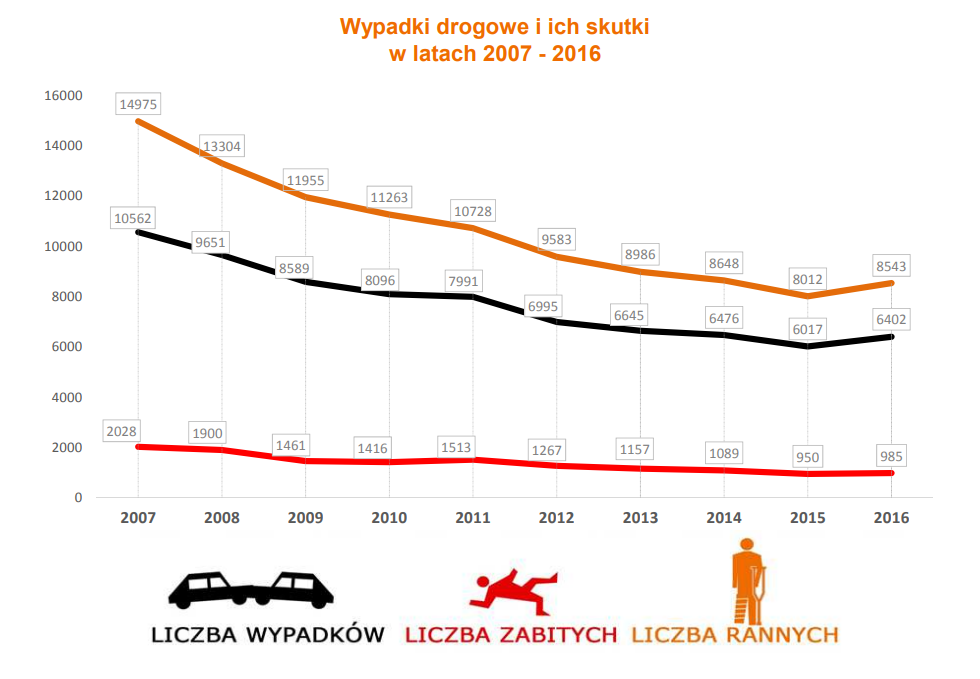
\includegraphics[width=1\textwidth]{picture1}
\source{Raport o stanie bezpieczeństwa ruchu drogowego dla dróg krajowych w zarządzie GDDKiA.}
\end{figure}

Z Rys. \ref{wypadkiSkutki} odczytać można, że liczba wypadków, z jednym wyjątkiem (z roku 2016) nieustannie maleje. W 2007 roku miało miejsce 10562 wypadków, w których liczba zabitych wyniosła 2028 osób, natomiast rannych było 14975. W porównaniu z 2016 został odnotowany spadek o ok. 40 \%. Niewątpliwie jest to ogromny sukces, jednak liczba ta dalej jest zatrważająco wysoka.


\section{Cele pracy}
\label{sec:celePracy}

Głównym celem niniejszej pracy dyplomowej było stworzenie inteligentnego systemu, mającego za zadanie predykcję dopuszczalnych prędkości w ruchu drogowym. Ponadto zostały opracowane modele i narzędzia pozwalające na obliczenie prędkości ma drogach. Rozwiązanie bazuje na metodach automatycznego wnioskowania, modelach matematycznych i informacjach geoprzestrzennych. Dzięki temu, możliwe było wyznaczenie optymalnego rozwiązania dla złożonego, wielokryterialnego problemu, w którym kluczowe znaczenie miało bezpieczeństwo uczestników ruchu drogowego, przy zachowaniu maksymalnej przepustowości infrastruktury drogowej.

Algorytm predykcji dopuszczalnych prędkości w ruchu drogowym wykorzystuje następujące informacje

\begin{itemize}
\item \textbf{pojedyncze poziome zakręty} - zostały podzielone na trzy grupy, według długości promienia skrętu:
 \begin{itemize}
 	\item \textbf{mały promień skrętu} - o maksymalnej długości promienia 300m
 	\item \textbf{średni promień skrętu} - o długości promienia powyżej 300m i poniżej 600m
 	\item \textbf{duży promień skrętu} - o długości promienia powyżej 600m
 \end{itemize}
\item \textbf{pobliże szkół i miejsc zabaw} - w takich przypadkach prędkość musiała zostać dobrana, aby kierowca bez przeszkód mógł zatrzymać się, nie powodując zagrożenia dla zdrowia i życia osób niepełnoletnich. Należy mieć na uwadze fakt, że zachowanie małoletnich osób często jest nieobliczalne. Nigdy nie wiadomo kiedy mogą pojawić się na drodze
\item \textbf{pobliże sklepów i miejsc kultów religijnych} - dostosowanie prędkości do większego niż zwykle ruchu pieszych jak i pojazdów mechanicznych.
\item \textbf{pobliże przystanków autobusowych i tramwajowych} - zdarzają się szczególne sytuacje, gdy pasażerowie komunikacji zbiorowej, bez uprzedniego upewnienia się, biegną  do już odjeżdżającego autobusu czy tramwaju. W takim przypadku szczególnie ważne jest dostosowanie prędkości, żeby kierowca mógł bez przeszkód, odpowiednio wcześniej, zareagować na taką ewentualność
\item \textbf{przejścia dla pieszych} - w sytuacjach jak powyżej, z tą różnicą, że zamiast na autobus, przebiegają na ''późnym zielonym'' lub czasem już czerwonym. Do takich sytuacji najczęściej dochodzi w miastach, gdzie tempo życia jest bardzo duże. Należy pamiętać, że ok. 25\% wypadków na przejściach z sygnalizacją spowodowane jest wtargnięciem pieszego na czerwonym świetle
\item \textbf{ilość pasów ruchu} - prędkość jest większa na kilku pasmowej drodze, w porównaniu z jednopasmową
\item \textbf{typ nawierzchni} - jest to bardzo ważny czynnik, ponieważ pojazdy mechaniczne, poruszając się z nieodpowiednią prędkością po nieprzystosowanej do tego nawierzchni, np. żwirowej, bardzo szybko ulegają kosztownym uszkodzeniom
\item \textbf{typ drogi} - w skład których wchodzą autostrady, drogi osiedlowe, ekspresowe, główne itp.
\item \textbf{zmiana prędkości między poszczególnymi strefami ograniczeń prędkości} - płynna jazda jest znacznie mniej ryzykowna niż nagła zmiana prędkości pojazdu. Dlatego w sytuacjach, gdy na drodzę znajduje się np. przejście dla pieszych, należy stopniowo ustawiać coraz to niższe wartości znaków sygnalizujących ograniczenie prędkości
\item \textbf{przejazdy kolejowe} - są zarówno strzeżone jak i niestrzeżone. W obu przypadkach należy zachować szczególną ostrożność, dlatego też prędkość musi być odpowiednio niższa. Trzeba mieć na uwadze, że przez dużą masę pojazdów szynowych, wypadki kolejowe należą do jednych z najbardziej śmiercionośnych.
\end{itemize}

Oprócz danych pobranych z OpenStreetMap, program posiada możliwość manualnego, przez zwykłego użytkownika, definiowania obiektów i przeszkód na drodze. Jest to szczególnie istotne, gdyż nie wszystkie dane umieszczone są w OSM.


Kluczową kwestią działanie algorytmu są również miejsca, w których powinien umieszczać znaki ograniczenia prędkości. Kierowca odpowiednio wcześniej musi zostać poinformowany o przeszkodzie na drodze, żeby mieć wystarczającą ilość czasu na reakcję. Dla przykładu, niedopuszczalna jest sytuacja, podczas której kierowca podróżując z szybkością 90 km/h, natrafia na znak informujący o znajdującym się za nim przejściu dla pieszych. Prawidłowo działający algorytm, powinien informować o potrzebie stopniowej redukcji prędkości, poprzez umieszczanie znaków ograniczeń prędkości o coraz to mniejszych wartościach. Dzięki temu możliwe jest zapewnienie płynność jazdy, przy zachowaniu odpowiedniego bezpieczeństwa.


%Raport o stanie bezpieczeństwa ruchu drogowego dla dróg krajowych w zarządzenie GDDKiA



\section{Wykorzystane technologie}
\label{sec:wykorzystaneTechnologie}
	Cała aplikacja bazuje na dynamicznej stronie internetowej. W tym celu został wykorzystany stos technologiczny, bazujący na javascripcie, jakim jest MEAN stack. Miałem kilka powodów, dla którym wybrałem te konkretne technologie. Pierwszym jest rosnąca popularność tego stosu. Coraz więcej firm przekonuje się do tej technologii, więc popyt na programistów z tego zakresu rośnie z roku na rok. Drugim powodem jest fakt, że można go uruchomić na prawie każdym urządzeniu czy platformie, dzięki czemu jest zapewniona duża przenośność kodu. Dodatkowo MEAN stack idealnie nadaje się do prostych, skalowalnych aplikacji webowych, w których nacisk kładziony jest na wymianę danych w czasie rzeczywistym na wielu urządzeniach.

	Back-end aplikacji został napisany w Node.js. Jego głównym zadaniem jest połączenie  się z mLabem w celu pobrania, zapisu, edycji i usuwania danych. Ponadto komunikuje się również z frontendem, po to, aby przekazywać pobrane dane.  Dodatkowo, w celu zmniejszenia objętości kodu i tym samym zwiększenia jego czytelności, został użyty framework Express.js.

	Za zarządzanie front-endem odpowiedzialny jest angular w wersji 5. Na nim została uruchomiona biblioteka Leaflet. Umożliwia ona wyświetlanie interaktywnej mapy, którą zasilić można różnymi typami danych, np. w formacie GeoJson. Dzięki niej, użytkownik zyskał możliwość wprowadzania swoich danych, przeglądania już istniejących czy zasięgnięcia informacji o dozwolonych prędkościach na danych odcinkach dróg. Kolejną,  istotną funkcjonalnością biblioteki Leaflet jest możliwość zarządzania wyświetlanymi obiektami. W prosty sposób można ukryć wszystkie dane, wyświetlać tylko drogi, tylko ograniczenia prędkości lub różne kombinację danych, które nas interesują.

\section{Przegląd literatury}
\label{sec:przegladLiteratury}

Han(2009) podaje przykład, jak zmiana prędkości wpływa na bezpieczeństwo i płynność jazdy. Jeśli kierowca napotka zbyt wiele stref prędkości z obrębie krótkiego odcinka drogi lub zbyt wiele zmian ograniczeń prędkości w sąsiedztwie danej strefy, to wtedy może poczuć dezorientację. Zwraca uwagę, jak ważne jest rozmieszczenie odpowiednich znaków, dla zredukowania poziomu stresu kierowcy.

Nama(2016) przedstawia jak kierowcy dostosowują prędkość w sytuacji gdy znajdują się na górzystej, nieregularnej drodze. Średnia wariancja prędkości w takim terenie wynosi ok. 55\%. Spowodowane jest to połączeniem cech geometrycznych zarówno poziomych jak i pionowych. Kierowcy na potrzeby bezpieczeństwa, w przypadku poziomych zakrętów, zmniejszają prędkość. Dodatkowym czynnikiem jest także ciągłe, zmieniające się nachylenie terenu. Uwzględnić należy również fakt, że zakręty znajdujące się na szczycie, wyglądają na znacznie bardziej niebezpieczne niż są w rzeczywistości. Wszystkie te czynniki w niekorzystny sposób wpływają na utrzymywanie stałej prędkości. Tabela \ref{predkosciPromienKrzywizny}. przedstawia średnią prędkość pojazdów w zależności od promienia krzywizny zakrętu, jego długości oraz nachylenia.


\begin{table}[ht]
\centering
\caption{Średnie prędkości pojazdów w zależności od promienia krzywizny, długości oraz nachylenia}
\label{predkosciPromienKrzywizny}
\begin{tabular}{| l | l | l | l | }
\hline
\textbf{promień krzywizny (m)} & \textbf{nachylenie (\%)} & \textbf{długość zakrętu (\%)} & \textbf{średnia prędkość (km/h)} \\ \hline
50 & 4 & 74 & 48.9\\ \hline
100 & 2 & 139 & 47.8\\ \hline
100 & -6 & 33 & 56.2\\ \hline
100 & 6 & 33 & 49.9\\ \hline
150 & -6 & 31 & 49.8\\ \hline
150 & -4 & 64 & 54.3\\ \hline
150 & 2 & 32 & 54.7\\ \hline
150 & 4 & 43 & 52.1\\ \hline
200 & -4 & 56 & 54.2\\ \hline
200 & -2 & 27 & 59.6\\ \hline
200 & 2 & 205 & 45.8\\ \hline
200 & 4 & 10 & 60.9\\ \hline
200 & 6 & 102 & 50.1\\ \hline
300 & -6 & 73 & 58.2\\ \hline
300 & 2 & 74 & 52.6\\ \hline

\end{tabular}
\source{Na podstawie Expanded Operating Speed Model}
\end{table}

W tabeli \ref{predkosciPromienKrzywizny} znalazły się dane z obserwacji na drodze, na której ograniczenie prędkości wynosiło 50 km/h. Zauważyć można, że w 45\% prędkość była wyższa niż  dopuszczalna.

Forbes(2012) wspomina o relacji pomiędzy prędkością, a ryzykiem wypadku dla prędkości pomiędzy 25 km/h a 120 km/h. Gdy średnia prędkość ruchu jest zmniejszona, liczba wypadków i  poziom niebezpieczeństwa spowodowania urazów prawie zawsze maleje. Gdy średnia prędkość ruchu wzrasta, liczba wypadków i poziom niebezpieczeństwa spowodowania urazów przeważnie rośnie. Relacja między średnią prędkością a ryzykiem wypadków może być adekwatnie opisana według poniższego modelu:

\begin{equation}
CMF = (V_a / V_b)^X
\end{equation}
gdzie
\begin{eqwhere}[2cm]
	\item[$CMF$] Współczynnik modyfikacji wypadku
	\item[$V_a$] średnia prędkość przed warunkiem
	\item[$V_b$] średnia prędkość po warunkiem
	\item[$X$] \begin{itemize}
		3.6 dla częstotliwości wypadków, w których pojawiły się ofiary śmiertelne

		2.0 dla częstotliwości wypadków, w których nie było ofiar śmiertelnych

		1.0 dla częstotliwości gdzie uszkodzeniu uległy tylko pojazdy

		4.5 dla ofiar śmiertelnych

		2.7 dla których poszkodowani ponieśli tylko obrażenia ciała
	\end{itemize}

\end{eqwhere}
Porównuje także ograniczenia prędkości dla poszczególnych obszarów znajdujących się w USA. Ich wynik znajduje się w tabeli \ref{ograniczeniaStany}.

\begin{table}[ht]
\centering
\caption{Ograniczenia prędkości w różnych stanach}
\label{ograniczeniaStany}
\begin{tabular}{|c|c|c|}
\hline
\textbf{Stan}                    & \textbf{Prędkość} & \textbf{Obszar} \\ \hline
\multirow{5}{*}{Delaware}   & 40 km/h & dowolna dzielnica biznesowa \\ \cline{2-3}
& 40 km/h & dowolna dzielnica mieszkalna \\ \cline{2-3}
& 30 km/h & wszystkie strefach szkolnych \\ \cline{2-3}
& 80 km/h & dwupasmowa jezdnia \\ \cline{2-3}
& 90 km/h & czteropasmowa jezdnia \\ \hline

\multirow{6}{*}{Minneasota}   & 15 km/h & alejki \\ \cline{2-3}
& 50 km/h & ulice dzielnic miejskich \\ \cline{2-3}
& 110 km/h & wiejskie autostrady międzystanowe \\ \cline{2-3}
& 105 km/h & miejskie autostrady międzystanowe \\ \cline{2-3}
& 105 km/h & drogi ekspresowe \\ \cline{2-3}
& 90 km/h & pozostałe drogi \\ \hline

\multirow{5}{*}{Oregon}   & 25 km/h & alejki, wąskie uliczki mieszkalne  \\ \cline{2-3}
& 30 km/h & dzielnice biznesowe, strefy szkolne \\ \cline{2-3}
& 40 km/h & dzielnice mieszkalne, parki publiczne, brzegi oceanu \\ \cline{2-3}
& 90 km/h & wiejskie autostrady, ciężarówki na międzystanowych autostradach \\ \cline{2-3}
& 105 km/h & pojazdy pasażerskie, lekkie ciężarówki na międzystanowych autostradach\\ \hline
\end{tabular}
\source{Na podstawie Methods and Practices for Setting Speed Limits: An Informational Report}
\end{table}


Han(2009) zwraca uwagę, jak pora dnia wpływa na ruch na drodzę. W godzinach porannych, gdy osoby pracujące jadą do pracy, osoby nieletnie do szkół oraz w godzinach popołudniowych, gdy wracają do domów. Obserwowany jest wzmożony ruch na drogach. Więcej pojazdów na drodze, oznacza większe korki, a co za tym idzie, zmniejszenie rzeczywistej prędkości. Natomiast w pozostałych porach dnia, gdy ruch jest mniejszy, możliwe jest szybsze poruszanie się po drodze. C. Han opisuje także jak prawidłowo ustawiać znaki drogowe. Oznakowanie powinno być umieszczone w każdym odpowiednim punkcie wzdłuż drogi, np. wokół potencjalnych punktów konfliktowych, zwężeniach i rozwidleniach dróg, zmianie ich nawierzchni itp. Powtórzenia znaków, najlepiej żeby były w odległości 1000m na autostradach. W obszarach miejskich, rekomendowana odległość to 400-500 m.

Jurewicz(2014) wskazuje bezpośrednią relację pomiędzy prędkością a ryzykiem wypadku. W sytuacji gdy prędkość jest zmniejszana,  liczba wypadków i rannych spada w 85 procentach przypadków. Gdy prędkość jest zwiększana, liczba wypadków i rannych wzrasta w 71 procentach przypadków. Największym dowodem na to są tak zwane badania 'przed i po'. W latach 1980 ograniczenie prędkości dla wiejskich i zewnętrznych autostrad w metropolii zostało zwiększone ze 100 km/h do 110 km/h, ale zostało  z powrotem zredukowane do 100 km/h z powodu obaw o bezpieczeństwo. Badanie 'przed, w trakcie i po' zostało prowadzone na przestrzeni 2,5 roku. W sytuacji, gdy ograniczenie prędkości zostało zwiększone do 110 km/h, wskaźnik ofiar wypadków wzrósł o prawie 25\%. Gdy prędkość ponownie została zmniejszona do 100 km/h wskaźnik zmalał o prawie 20\%.

Vadeby i Frosman (2018) przeprowadzili badania na temat, jak nowe ograniczenia prędkości wpłynęły na bezpieczeństwo. Dla przykładu, gdy na wiejskich drogach została zmniejszona wartość dozwolonej prędkości z 90 km/h do 80 km/h, zauważono spadek liczby wypadków śmiertelnych o 14 w skali roku. Nie zauważono natomiast żadnych znaczących zmian dla liczby poważnych obrażeń ciała. Na autostradzie, po zwiększeniu dozwolonej prędkości do 120 km/h, zanotowano wzrost wypadków, w których doszło do poważnych obrażeń. Nie odnotowano natomiast znaczącej zmiany względem ofiar śmiertelnych. Wzrost liczby poważnych obrażeń ciała wystąpił na wszystkich rodzajach autostrad, jednak największy wzrost został zauważony na wąskich autostradach o szerokości 21.5 m. Dla dwupasmowych jezdni, po zmniejszeniu prędkości ze 110 do 100 km/h, doszło do zmniejszenia liczby wypadków z poważnymi obrażeniami ciała o 16 w skali roku. Vadeby i Frosman (2018) wskazują także na fakt, iż wzrost dozwolonej prędkości o 10 km/h spowodował średni wzrost prędkości pojazdów mechanicznych o ok. 2-3 km/h, a zmniejszenie dozwolonej prędkości o 10 km/h, spowodował zmniejszenie średniej prędkości pojazdów o 3 km/h.

Soriguera i inni (2017) przeprowadzili badanie, które wykazało, jak mała wartość ograniczenia prędkości wpływa na ruch uliczny. Jako rezultat, uzyskali następujące wyniki.

\begin{itemize}
\item Dla ograniczenia prędkości do 80 km/h, maksymalna przepustowość może wynieść 1972 samochodów na godzinę na jednym pasie ruchu, dla szerokiego zakresu zajętości jezdni (17.6 - 25.8\%) i średniej prędkości wahającej się między 51 a 73 km/h
\item Dla ograniczenia prędkości do 60 km/h, maksymalna przepustowość nie uległa dużej zmianie, wyniosła 1956 pojazdów na godzinę na jednym pasie ruchu. Zajętość jezdni utrzymywała się na wysokim poziomie 24.4 - 25.8\%.
\item Dla ograniczenia prędkości do 40 km/h, maksymalna przepustowość nieznacznie zmalała, do poziomu 1942 samochodów na godzinę na jednym pasie ruchu. Natomiast znacznie wzrosła zajętość jedni, wynosiła 32.0 - 34.7\%.
\end{itemize}

Z powyższych wyników, można dojść do dwóch wniosków. Pierwszy jest taki, że zmniejszenie prędkości skutkuje znacznym zwiększeniem poziomu zajętości jezdni w warunkach swobodnego przepływu. W skrócie, zmniejszenie prędkości pozwala osiągnąć stabilny, wysoki poziom zajętości jezdni, zapobiegając tym samym różnym wypadkom i utrzymywaniem dużej akumulacji pojazdów na drodze. Drugi wniosek jest taki, że dla małej prędkości, jaką jest 40 km/h, średnia prędkość przepływu pojazdów, wynosząca 1942 pojazdów/h/pas, może zostać podtrzymana przez dłuższy okres. W praktyce oznacza to znaczne zmniejszenie prawdopodobieństwa wystąpienia korków na drodze.

\section{Układ pracy}
\label{sec:ukladPracy}

Praca składa się z 5 rozdziałów.

\begin{itemize}
\item Pierwszy z nich składa się ze wstępu, celów pracy, wykorzystanych technologii oraz przeglądu literatury.
\item W drugin rozdziale zawarto opracowanie teoretyczne poszczególnych części algorytmu. Przestawiono również ogólny schemat, sposób w jaki algorytm pobiera dane, skąd je bierze oraz jak je parsuje, przetwarza i wyświetla na stronie.
\item Trzeci rodział zawiera wyniki działania algorytmu dla poszczególnych jego składowych
\item W piątym rozdziale został umieszczony opis interfejsu użytkownika
\end{itemize}

\chapter{Algorytm - TODO}
\label{cha:Algorytm}

Niniejszy rozdział skupiać się będzie na algorytmie służącym do rozwiązania problemu, jakim jest wyznaczenie optymalnej prędkości na drodze. Zostaną w nim opisane poszczególne składowe wchodzące w jego skład, takie jak:
\begin{itemize}
\item przyporządkowanie obiektów reprezentowanych przez punkty, do poszczególnych dróg
\item przyporządkowanie obiektów reprezentowanych przez dwuwymiarowe figury geometryczne, do poszczególnych dróg
\item wyznaczanie dopuszczalnej prędkości
\item odpowienie umiejscowienie znaków
\end{itemize}

Dodatkowo, w celu lepszej wizualizacji problemu, zostaną umieszczone zdjęcia, przedstawiające działanie poszczególnych części algorytmu.

\newpage
\section{Przyporządkowanie obiektów reprezentowanych przez punkty, do poszczególnych dróg}
\label{sec:ObiektyPunktDrogi}

Jednym z kluczowych elementów działania algorytmu jest odpowiednie przyporządkowanie obiektów drogowych do poszczególnych dróg. W OpenStreetMap reprezentowane są zarówno przez punkty, jak również przez dwuwymiarowe obiekty geometryczne.


Obiekty z OpenStreetMap reprezentowane przez punkty:
\begin{itemize}
\item przejścia dla pieszych
\item przejazdy kolejowe
\item sygnalizacja świetlna
\end{itemize}


W niniejszej sekcji skupię się na rozwiązaniu problemu jakim jest przyporządkowanie obiektów przedstawianych jako punkty, do poszczególnych dróg. Do tego celu wykorzystam wzór \ref{eq:distancePointLineal}, wyznaczający odległość punktu od prostej.

\begin{figure}[h]
\centering
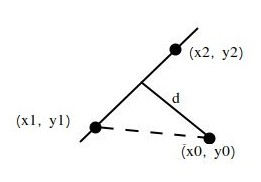
\includegraphics[width=0.5\textwidth]{dlugoscPktOdProstej}
\source{Na podstawie mathworld.wolfram.com}
\end{figure}

Wzór wyznaczający odległość punktu od prostej:

\begin{equation} \label{eq:distancePointLineal}
d = \frac{| (x_2 - x_1)(y_1 - y_0) - (x_1 - x_0)(y_2 - y_1) |}{\sqrt{(x_2 - x_1)^2 + (y_2 - y_1)^2}}
\end{equation}\newline

\begin{itemize}
\item Zmienne: x1, y1, x2, y2 oznaczają współrzędne geograficzne odpowiednio początku i końca drogi.
\item Zmienne x0, y0 oznaczają współrzędne punktu reprezentujące obiekt drogowy.
\item Zmienna d oznacza najkrótszą odleglość punktu od drogi.
\end{itemize}


\newpage
\section{Wyznaczanie współrzędnych punktu znajdującego się na drodze, odległego o n metrów od innego punktu}
\label{sec:pointCoordinatesFromAnotherPoint}

Istotnym aspektem działania algorytmu jest rozwiązanie problemu wyznaczenie współrzędnych punktu, znajdującego się na drodze, odległego o n metrów od innego punktu.  Jest to niezbędne w sytuacji, gdy np. program musi ustawić na drodze znak ograniczenia prędkości w odległosci n metrów od przejścia dla pieszych.

Do rozwiązania tego zadania, posłużyłem się własnościami trygonometrycznymi.


\begin{figure}[h]
\centering
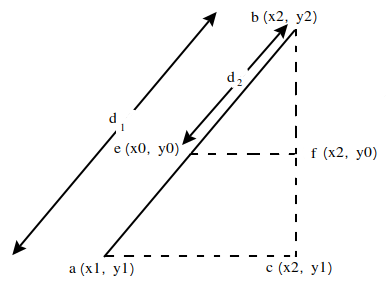
\includegraphics[width=0.5\textwidth]{distance}
\end{figure}

Odległość między dwoma punktami a i b wynosi:
\begin{equation}
d_1 = \sqrt{(x1 - x2)^2 + (y1 - y2)^2}
\end{equation}\newline

oraz sinus kąta abc:
\begin{equation}
sin_{abc} = \frac{x2 - x1}{d_1}
\end{equation}\newline

jak również sinus kąta ebf:
\begin{equation}
sin_{ebf} = \frac{x2 - x0}{d_2}
\end{equation}\newline

oraz to, że sinusy tego samego kąta są równe:
\begin{equation}
sin_{abc} = sin_{ebf} => \frac{x2 - x1}{d_1} = \frac{x2 - x0}{d_2}
\end{equation}\newline

przez proste przekształcenie, otrzymujemy wzór na współrzędną x0

\begin{equation}
x0 = x2 - \frac{d_2*(x2 - x1)}{d_1}
\end{equation}\newline

Wyznaczenie wzoru na współrzędną y0 jest podobne do wyznaczania współrzędnej x0, z tą różnicą, że zamiast sinusa, liczymy cosinusa kąta abc:

\begin{equation}
cos_{abc} = \frac{y2 - y1}{d_1}
\end{equation}\newline

oraz cosinusa kąta ebf:
\begin{equation}
cos_{ebf} = \frac{y2 - y0}{d_2}
\end{equation}\newline

a skoro cosinus tego samego kąta są równe:
\begin{equation}
cos_{abc} = cos_{ebf} => \frac{y2 - y1}{d_1} = \frac{y2 - y0}{d_2}
\end{equation}\newline

otrzymujemy równanie współrzędnej y0:
\begin{equation}
y0 = y2 - \frac{d_2*(y2 - y1)}{d_1}
\end{equation}\newline

Przez powyższe obliczenia, wyznaczone zostały wspórzędne poszukiwanego punktu:

\begin{equation} \label{eq:calculatedCoordinates}
(x2 - \frac{d_2*(x2 - x1)}{d_1}, y2 - \frac{d_2*(y2 - y1)}{d_1})
\end{equation}\newline

\newpage
\section{Wyznaczanie minimalnego obszaru pokrywającego}

W niniejszej sekcji skupię się na sposobie w jaki algorytm wyznacza minimalny obszar pokrywający (eng. minimum bounding box). Będzie on wykorzystany w późniejszych obliczeniach, mających na celu przypisanie poszczególnych dróg do danych obszarów, na których obowiązuje ograniczenie prędkości.

Rys. \ref{sec:minBoundingBoxFirst} przedstawia przykładowy wielokąt reprezentujący interesujący nas obiekt pobrany z OpenStreetMap.

\begin{figure}[h]
\caption{Przykładowy wielokąt reprezentujący obiekt na mapie}
\label{sec:minBoundingBoxFirst}
\centering
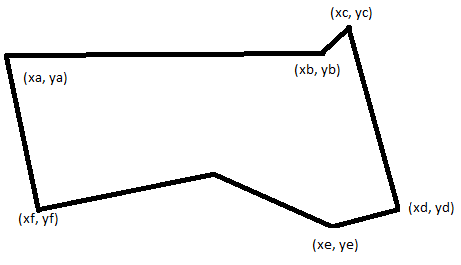
\includegraphics[width=0.8\textwidth]{minBoundingBoxFirst}
\end{figure}

W celu znalezienia minimalnego obszaru pokrywający niezbędne jest wyznaczenie czterech współrzędnych (x1, y1), (x2, y2), (x3, y3), (x4, y4) reprezentuących cztery wierzchołki prostokąta.

W celu wyznaczenia wierzchołka północno-zachodniego, należy obliczyć minimalną wartość współrzędnej x oraz maksymalną wartość współrzędnej y.

\begin{equation} \label{sec:drugiWierzcholek}
\begin{split}
x1 = min(x_a, x_b, x_c, x_d, x_e, x_f, x_g) \\
y1 = min(y_a, y_b, y_c, y_d, y_e, y_f, y_g)
\end{split}
\end{equation}\newline

Żeby wyznaczyć wierzchołek północno-wschodni, należy obliczyć maksymalną wartość współrzędnej x i y.
\begin{equation} \label{sec:trzeciWierzcholek}
\begin{split}
x2 = max(x_a, x_b, x_c, x_d, x_e, x_f, x_g)  \\
y2 = max(y_a, y_b, y_c, y_d, y_e, y_f, y_g)
\end{split}
\end{equation}\newline

Wierzchołek południowo-wschodni obliczamy jako maksymalną wartość współrzędnej x oraz minimalną wartość wsółrzędnej y.
\begin{equation} \label{sec:czwartyWierzcholek}
\begin{split}
x3 = max(x_a, x_b, x_c, x_d, x_e, x_f, x_g) \\
y3 = min(y_a, y_b, y_c, y_d, y_e, y_f, y_g)
\end{split}
\end{equation}\newline

Aby wyznaczyć południowo-zachodni wierzchołek, należy obliczyć minimalną wartość współrzędnej x i y.

\begin{equation} \label{sec:pierwszyWierzcholek}
\begin{split}
x4 = min(x_a, x_b, x_c, x_d, x_e, x_f, x_g) \\
y4 = min(y_a, y_b, y_c, y_d, y_e, y_f, y_g)
\end{split}
\end{equation}\newline

Po wyznaczeniu powyższych współrzędnych minimalny obszar pokrywający wygląda tak, jak na rysunku \ref{sec:secondtBB}


\begin{figure}[h]
\caption{Minimalny obszar pokrywający dany obiekt}
\label{sec:secondtBB}
\centering
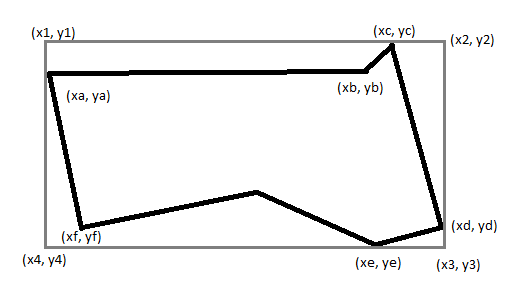
\includegraphics[width=0.9\textwidth]{minBoundingBox}
\end{figure}

\newpage
\section{Powiększanie wyznaczonego obszaru pokrywającego}

Kolejnym krokiem niezbędnym do przyporządkowania dwuwymiarowych obiektów do poszczególnych dróg jest powiększenie wyznaczonego obszaru pokrywającego. W celu wyznaczenia wierzchołków powiększonego obszaru, skorzystam z poniżej podanych równań.

\begin{equation}
\begin{split}
x1' = x1 - n \\
y1' = y1 + n \\
\end{split}
\end{equation}

\begin{equation}
\begin{split}
x2' = x2 + n \\
y2' = y2 + n \\
\end{split}
\end{equation}

\begin{equation}
\begin{split}
x3' = x3 + n \\
y3' = y3 - n \\
\end{split}
\end{equation}

\begin{equation}
\begin{split}
x4' = x4 - n \\
y4' = y4 - n \\
\end{split}
\end{equation}

Rys. \ref{sec:thirdBB} przedstawia minimalny obszar pokrywający powiększony o n metrów względem pierwotnego. Oczywiście obszar można dowolnie powiększać, w zależności od obiektu, który się w nim znajduje. Tak więc dla placów zabaw czy przedszkoli będzie znacznie większy, w porównaniu do np. przystanków autobusowych.

\begin{figure}[h]
\caption{Minimalny obszar pokrywający dany obiekt powiększony o n metrów}
\label{sec:thirdBB}
\centering
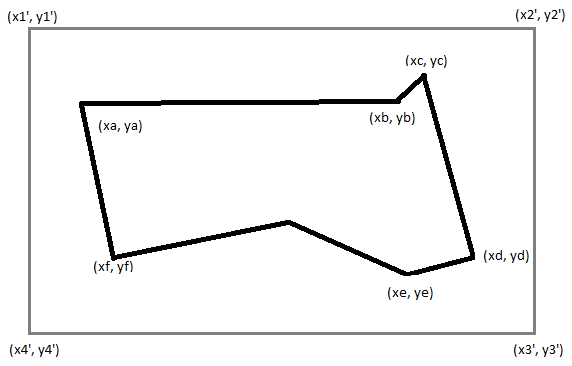
\includegraphics[width=0.7\textwidth]{BoundingBoxExtended}
\end{figure}

\newpage
\section{Łączenie powiększonych obszarów pokrywających}

W celu przyszpieszenia części algorytmu odpowiedzialnego za przypisywanie danego odcinka drogi do obszaru w którym obowiązuje ograniczenie prędkości, niezbędne jest połączenie nachodzących na siebie obszarów oraz wyznaczenie jego konturu. Można rozróżnić kilka przypadków:
\begin{itemize}
\item gdy jeden obszar całkowicie znajduje się wewnątrz drugiego
\item gdy dwa rogi obszaru mającego kształt prostokątu znajdują się wewnątrz innego obszaru
\item gdy tylko jeden róg obszaru mającego kształt prostokątu znajdje się wewnątrz innego obszaru
\end{itemize}
W niniejszych podrozdziale skupię na dokładnej metodzie wyznaczania konturu dla każdego z powyższych przypadków.

\subsection{Łączenie powiększonych obszarów pokrywających w przypadku gdy jeden obszar w całości znajduje się w drugim}

Do sytuacji w której dany obszar pokrywający w całości znajduje się wewnątrz innego obszaru dochodzi gdy np. wokół przedszkola znajduje się plac zabaw. W takiej sytuacji
można pominąć wewnętrzy obszar. Na rys \ref{fig:boundingBoxInside} został przedstawiony taki przypadek.

\begin{figure}[h]
\caption{Obszar pokrywający wewnątrz innego obszaru}
\label{fig:boundingBoxInside}
\centering
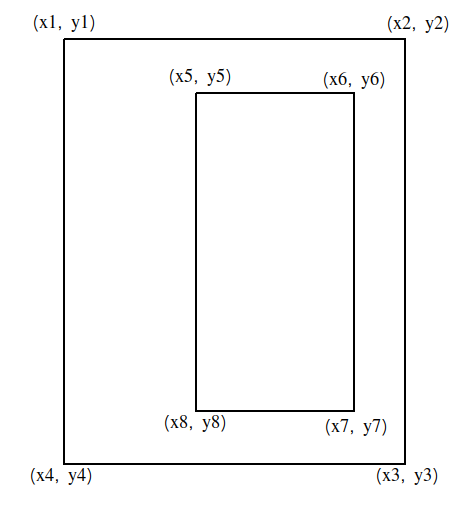
\includegraphics[width=0.6\textwidth]{boundingBoxInside}
\end{figure}

W pierwszym kroku należy znaleźć takie obszary. W tym celu algorytm iteruje po wszystkich obszarach i sprawdza, czy współrzędne spełniają wszystkie niżej przedstawione warunki.

\begin{equation}
\begin{split}
x4 <= x5 <= x2 \\
x4 <= x7 <= x2 \\
y4 <= y5 <= y2 \\
y4 <= x7 <= y2
\end{split}
\end{equation}

W następnym kroku algorytm usuwa tak znaleziony obszar. W wyniku czego na mapie pozostaje tylko obszar przestawiony na rys.\ref{fig:boundingBoxInsideRemoved}

\begin{figure}[h]
\caption{Wynik usunięcia obszaru pokrywającego wewnątrz innego obszaru}
\label{fig:boundingBoxInsideRemoved}
\centering
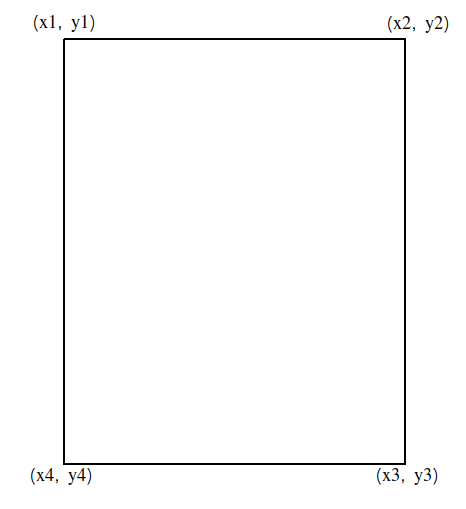
\includegraphics[width=0.6\textwidth]{boundingBoxInsideRemoved}
\end{figure}

\newpage
\subsection{Łączenie powiększonych obszarów pokrywających w przypadku gdy jeden obszar nachodzi w całości tylko jednym bokiem }

W przypadku gdy jeden obszar pokrywający w całości nachodzi tylko jednym bokiem, algorytm rozróżnia cztery możliwe sytuacje. Wszystkie one zostały przestawione na rysunku \ref{fig:OneSideBounding}.



\begin{figure}[h]
\caption{Wszystkie możliwe sytuacje w których jeden obszar nachodzi na drugi tylko jednym  bokiem}
\label{fig:OneSideBounding}
\centering
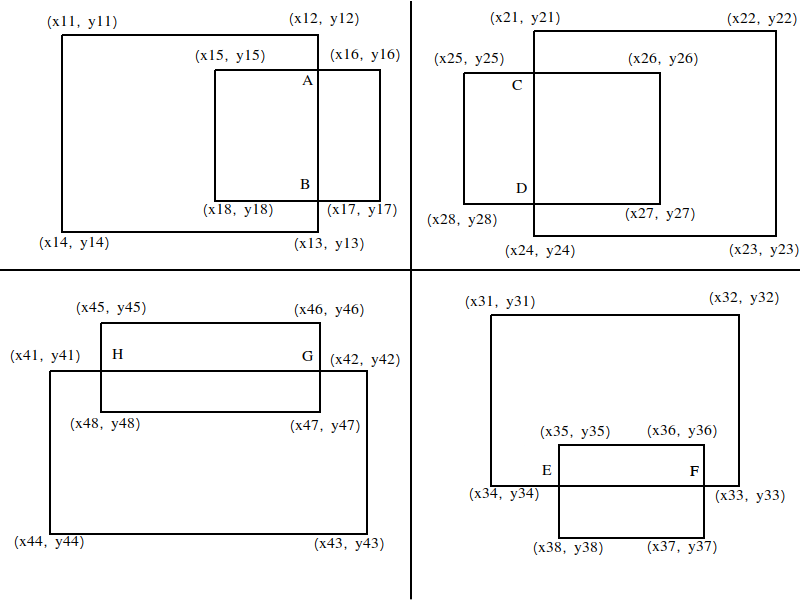
\includegraphics[width=0.8\textwidth]{OneSideBounding}
\end{figure}

W pierwszym kroku należy znaleźć takie obszary. W tym celu algorytm iteruje po wszystkich obszarach i sprawdza, czy współrzędne spełniają wszystkie niżej przedstawione warunki.

Dla pierwszej ćwiarki z rys. \ref{fig:OneSideBounding}
\begin{equation}
\begin{split}
x11 <= x15 <= x13 \\
y13 <= y15 <= y11 \\
y13 <= y18 <= y11 \\
x13 < x16 \\
\end{split}
\end{equation}

Dla drugiej ćwiarki z rys. \ref{fig:OneSideBounding}
\begin{equation}
\begin{split}
x24 <= x26 <= x22 \\
y23 <= y26 <= y21 \\
y23 <= y27 <= y21 \\
x25 < x21 \\
\end{split}
\end{equation}

Dla trzeciej ćwiarki z rys. \ref{fig:OneSideBounding}
\begin{equation}
\begin{split}
x31 <= x35 <= x33 \\
x31 <= x36 <= x33 \\
y33 <= y35 <= y11 \\
y38 < x34 \\
\end{split}
\end{equation}

Dla czwartek ćwiarki z rys. \ref{fig:OneSideBounding}
\begin{equation}
\begin{split}
x41 <= x48 <= x43 \\
x41 <= x47 <= x43 \\
y43 <= y47 <= 411 \\
y46 > x42 \\
\end{split}
\end{equation}

W następnym kroku algorytm wyznacza punkty przecięcia. Z racji tego, że nachodzące obszary są prostokątami zrotowanymi pod takim samym kątem, to do ich wyznaczenia pobiera odpowiednie współrzędne już wyznaczonych obszarów.

Dla pierwszej ćwiarki z rys. \ref{fig:OneSideBounding}

\begin{equation}
\begin{split}
A = (x12, y15) \\
B = (x12, y16)
\end{split}
\end{equation}

Dla drugiej ćwiarki z rys. \ref{fig:OneSideBounding}

\begin{equation}
\begin{split}
C = (x21, y25) \\
D = (x21, y28)
\end{split}
\end{equation}

Dla trzeciej ćwiarki z rys. \ref{fig:OneSideBounding}

\begin{equation}
\begin{split}
E = (x35, y34) \\
F = (x36, y34)
\end{split}
\end{equation}


Dla czwartej ćwiarki z rys. \ref{fig:OneSideBounding}

\begin{equation}
\begin{split}
G = (x46, y42) \\
H = (x45, y42)
\end{split}
\end{equation}

W ostatnim kroku algorytm wyznacza kontur tak przygodowanej figury, poprzez połączenie współrzędnych w odpowiedniej kolejności. Zostało to przedstawione w poniższym równaniu:

Dla pierwszej ćwiarki z rys. \ref{fig:OneSideBounding}

\begin{equation}
\begin{split}
(x11, y11) -> (x12, y12) -> (x12, y15) -> (x16, y16) ->  \\
(x17, y17) -> (x12, y16) -> (x13, y13) -> (x14, y14)
\end{split}
\end{equation}

Dla drugiej ćwiarki z rys. \ref{fig:OneSideBounding}

\begin{equation}
\begin{split}
(x21, y21) -> (x22, y22) -> (x23, y23) -> (x24, y24) ->  \\
(x21, y28) -> (x28, y28) -> (x25, y25) -> (x21, y25)
\end{split}
\end{equation}

Dla trzeciej ćwiarki z rys. \ref{fig:OneSideBounding}

\begin{equation}
\begin{split}
(x31, y31) -> (x32, 312) -> (x33, y33) -> (x36, y34) ->  \\
(x37, y37) -> (x38, y38) -> (x35, y34) -> (x34, y34)
\end{split}
\end{equation}

Dla czwartej ćwiarki z rys. \ref{fig:OneSideBounding}

\begin{equation}
\begin{split}
(x41, y41) -> (x45, y42) -> (x45, y45) -> (x46, y46) ->  \\
(x46, y42) -> (x42, y42) -> (x43, y43) -> (x44, y44)
\end{split}
\end{equation}

W wyniku powyższego algorytmu, zostały wyznaczone kontury nachodzących na siebie obszarów. Zostały przedstawione na rys. \ref{fig:OneSideBoundingRemoved}

\begin{figure}[h]
\caption{Obrys nachodzących na siebie obszarów}
\label{fig:OneSideBoundingRemoved}
\centering
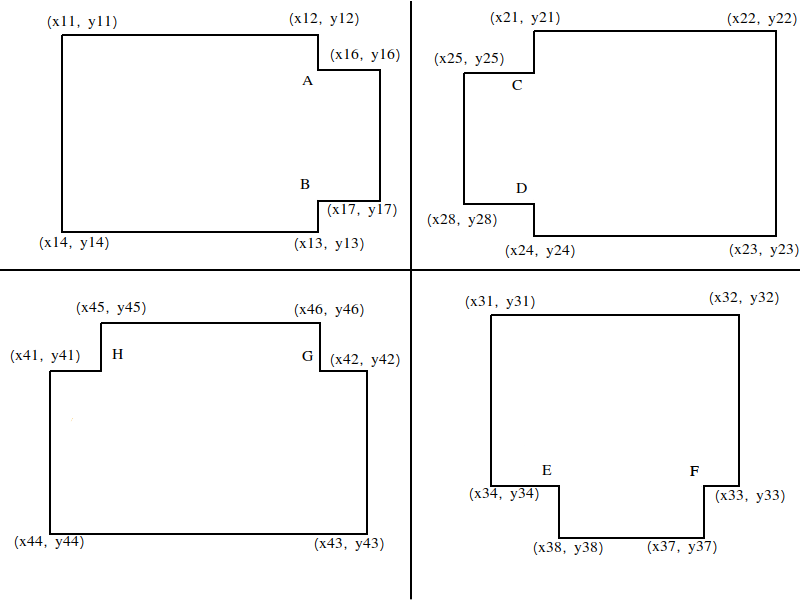
\includegraphics[width=0.75\textwidth]{OneSideBoundingRemoved}
\end{figure}

\newpage
\section{Przyporządkowanie obiektów reprezentowanych przez wielokąty, do poszczególnych dróg}
\label{sec:polygonLineDistance}

W niniejszej sekcji skupię się na rozwiązaniu problemu przyporządkowania obiektów reprezentowanych przez wielokątny do poszczególnych dróg. Wykorzystywane jest w sytuacjach, gdy trzeba określić dokładne współrzędne początku i końca strefy, na której obowiązuje ograniczonej prędkości. Obiekty na mapie, reprezentowane przez wielokąty:
\begin{itemize}
\item szkoły
\item parki
\item place zabaw
\item przystanki autobusowe i tramwajowe
\item sklepy
\item miejsca kultu
\end{itemize}




W pierwszej kolejności algorytm znajduje minimalny obszar pokrywający (eng. minimum bounding box) dany obiekt. W tym celu

\subsection{Powiększanie wyznaczonego obszaru pokrywającego}

Następnym krokiem jest powiększenie tak wyznaczonego obszaru o n metrów. Dzięki takiemu zabiegowi, możliwe będzie wyznaczenie strefy ogroniczonej prędkości.




\subsection{Łączenie powiększonych obszarów pokrywających}

W celu przyszpieszenia części algorytmu odpowiedzialnego za przypisywanie danego odcinka drogi do obszaru w którym obowiązuje ograniczenie prędkości, niezbędne jest połączenie nachodzących na siebie obszarów oraz wyznaczenie jego konturu. Można rozróżnić kilka przypadków:




\subsection{Wyznaczanie obszarów drogi znajdujących się w pobliżu interesującego nas obiektu}

Ostatnim krokiem jest wyliczenie, które drogi znajdują się o obrębie danego obszaru. Należy zaznaczyć, że Open Street Map, w przypadku łuków czy zakrętów, przedstawia je jako zbiór odcinków. Możemy tutaj wyróżnić dwa przypadki:
\begin{itemize}
\item żaden ze zbioru odcinków nie należy do danego obszaru
\item jeden lub pewna część odcinków znajduje się w obrębie danego obszaru. W takiej sytuacji należy wyznaczyć wszystkie współrzędne przecięcia, a później określić interesujące nas fragmenty drogi.
\end{itemize}


\subsubsection{Znajdowanie punktów przecięcia}

W celu znalezienia punktów przecięcia, wykorzystam fakt, że droga reprezentowana jest zbiór odcinków, oraz że interesujący nas obszar jest prostokątem - a więc posiada cztery boki.

W pierwszej kolejności algorytm będzie iterował po zbiorze odcinków. Każdy odcinek lub bok prostokąta reprezentowany jest przez dwie współrzędne:

\begin{equation}
\begin{split}
(x_a, y_a) \\
(x_b, y_b) \\
\end{split}
\end{equation}

Dzięki temu, bez problemu można określić równanie prostej przechodzącej przez te dwa punkty:

\begin{equation}
(y - y_a) (x_b-x_a) - (y_b - y_a) (x - x_a) = 0
\end{equation}

Oraz równanie w postaci kierunkowej:

\begin{equation} \label{sec:prostaKierunkowa}
y=\frac{y_a - y_b}{x_a - x_b}x + (y_a - \frac{y_a - y_b}{x_a - x_b}x_a)
\end{equation}

W celu wyznaczenia współrzędnej x punktu przecięcia wystarczy porównać oba równania:

\begin{equation}
\frac{y_c - y_d}{x_c - x_d}x + (y_c - \frac{y_c - y_d}{x_c - x_d}x_c)=\frac{y_a - y_b}{x_a - x_b}x + (y_a - \frac{y_a - y_b}{x_a - x_b}x_a)
\end{equation}

W wyniku czego otrzymujemy:

\begin{equation}
x = \frac{(y_a - \frac{y_a - y_b}{x_a - x_b}x_a) - (y_c - \frac{y_c - y_d}{x_c - x_d}x_c)}{\frac{y_c - y_d}{x_c - x_d} - \frac{y_a - y_b}{x_a - x_b}}
\end{equation}

Aby wyznaczyc współrzędną y, należy przekształcić równanie \ref{sec:prostaKierunkowa} do postaci:

\begin{equation}
x=\frac{y - (y_a - \frac{y_a - y_b}{x_a - x_b}x_a)}{\frac{y_a - y_b}{x_a - x_b}}
\end{equation}

Następnie porównać równania obu prostych:

\begin{equation}
\frac{y - (y_a - \frac{y_a - y_b}{x_a - x_b}x_a)}{\frac{y_a - y_b}{x_a - x_b}}=\frac{y - (y_c - \frac{y_c - y_d}{x_c - x_d}x_c)}{\frac{y_c - y_d}{x_c - x_d}}
\end{equation}

W wyniku czego otrzymujemy wzór na współrzędną y przecinającą obie proste:
\begin{equation}
y = \frac{(y_a - \frac{y_a - y_b}{x_a - x_b}x_a)(\frac{y_c - y_d}{x_c - x_d}) - (\frac{y_a - y_b}{x_a - x_b})(y_c - \frac{y_c - y_d}{x_c - x_d}x_c)}
{(\frac{y_c - y_d}{x_c - x_d})(\frac{y_a - y_b}{x_a - x_b})}
\end{equation}

\subsubsection{Sprawdzanie, czy punkt przecięcia należy do odcinka}

W celu sprawdzenia, czy punkt przecięcia należy do odcinka, posłużę się własnością, że suma długości mierzonej od początku odcinka do danego punktu oraz od danego punktu, do końca odcinka jest równa całkowitej długości odcinka.

\begin{equation} \label{eq:pointInSegment}
|AC| + |CB| = |AB|
\end{equation}

W celu lepszego zobrazowania, posłuże się rysunkiem \ref{sec:pointSegment}

\newpage
\begin{figure}[h]
\caption{Punkt wewnątrz odcinka}
\label{sec:pointSegment}
\centering
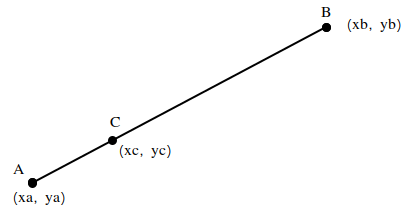
\includegraphics[width=0.6\textwidth]{pointInSegment}
\end{figure}

Odległość między dwoma punktami a i b wynosi:
\begin{equation}
d = \sqrt{(x1 - x2)^2 + (y1 - y2)^2}
\end{equation}\newline

Długość odcinka AC wynosi:

\begin{equation} \label{eq:distanceBetweenTwoPointAC}
d_{AC} = \sqrt{(xa - xc)^2 + (ya - yc)^2}
\end{equation}\newline

Długość odcinka CB wynosi:
\begin{equation} \label{eq:distanceBetweenTwoPointCB}
d_{CB} = \sqrt{(xc - xb)^2 + (yc - yb)^2}
\end{equation}\newline

Oraz długość odcinka AB wynosi:
\begin{equation}
d_{AB} = \sqrt{(xa - xb)^2 + (ya - yb)^2}
\end{equation}\newline

Zgodnie z równaniem \ref{eq:pointInSegment}, aby punkt nalezał do odcinka, musi spełniać warunek:

\begin{equation}
\sqrt{(xa - xb)^2 + (ya - yb)^2} = \sqrt{(xa - xb)^2 + (ya - yb)^2} + \sqrt{(xc - xb)^2 + (yc - yb)^2}
\end{equation}\newline

\subsubsection{Wyznaczenie obszarów drogi znajdujących się w pobliżu danego obiektu}



\newpage
\begin{figure}[h]
\caption{Droga przebiegająca przez wybrany obszar}
\label{sec:fourthBB}
\centering
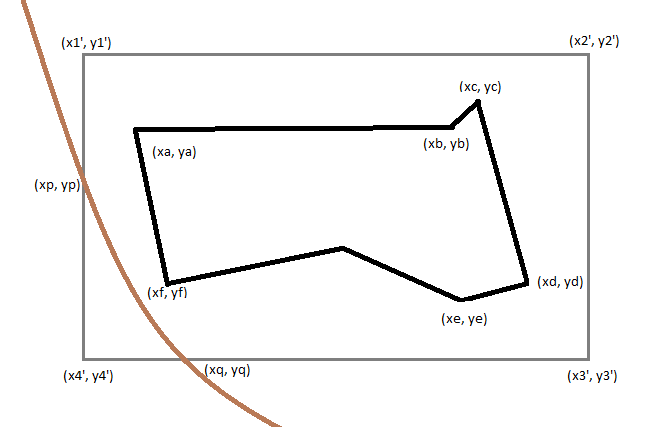
\includegraphics[width=0.8\textwidth]{minBoundingBoxWay}
\end{figure}

\newpage
\section{Przejścia dla pieszych}
\label{sec:pedestrialCrossing}
\subsection{Przyporządkowywanie przejść dla pieszych do poszczególnych dróg}

Bardzo ważnym czynnikiem doboru prędkości jest obecność przejść dla pieszych. Te z sygnalizacją świetlną nie stanowią problemu, ponieważ ruch pieszych poruszających się na nich jest ograniczony tylko do sytuacji, gdy sygnalizacja świeci się na zielono. W przypadku przejść bez sygnalizacji, sprawa się komplikuje, ponieważ kierowca jest zobowiązany do zachowania szczególnej ostrożności i zmiejszenia prędkości od 30 km/h.

Do przyporządkowania przejść dla pieszych, do poszczególnych dróg, posłużyłem się wzorem \ref{eq:distancePointLineal} na odległość punktu od prostej, przedstawionym w sekcji \ref{sec:ObiektyPunktDrogi}.


Rezultatem wdrożenia powyższego wzoru do programu, są:
\begin{itemize}
\item na niebiesko zaznaczone drogi, na których znajdują się przejścia dla pieszych
\item znakiem ''D-6'' zostały oznaczone przejścia dla pieszych
\end{itemize}
Wynik został przedstawiony na Rys. \ref{sec:PrzejscieDrogi}:

\begin{figure}[h]
\caption{Drogi na których znajdują się przejścia dla pieszych.}
\label{sec:PrzejscieDrogi}
\centering
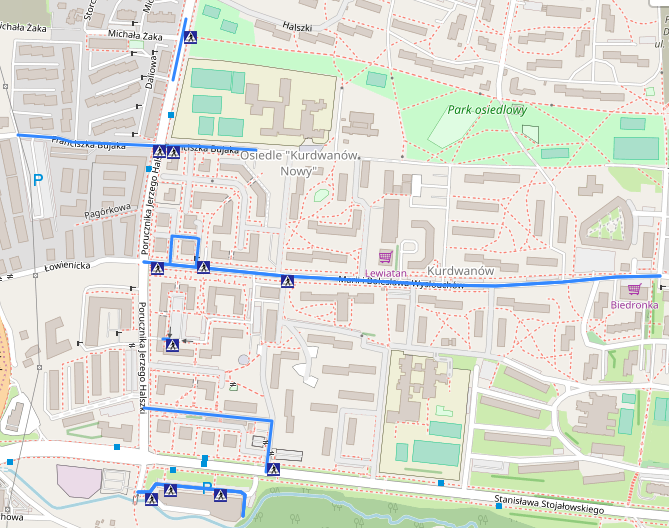
\includegraphics[width=0.9\textwidth]{PrzejscieDrogi}
\end{figure}

Dzięki tak zobrazowanej sytuacji, można ocenić skuteczność algorytmu przyporządkowującego przejścia dla pieszych do określonych dróg.

\subsection{Wyznaczanie prędkości i umieszczanie jej w odpowiednim miejscu na mapie}

Bezpieczna prędkość w pobliżu nieoznakowanych przejść dla pieszych wynosi ok. 30 km/h. Zapewnia ona zarówno wystarczajacy czas reakcji, odpowiednio krótką drogę hamowania oraz zmiejsza ryzyko wystąpień potrąceń pieszych.

Algorytm umieszcza znaki ograniczenia prędkości:
\begin{itemize}
\item w odległości 50 m od przejścia, gdy maksymalna prędkość na drodze wynosi 60 km/h
\item w odległości 150 m od przejścia, gdy maksymalna prędkość przekracza 60 km/h
\item w przypadku, gdy przejście dla pieszych znajduje się w odległości mniejszej niż 50m lub 150m (w zależności od maksymalnej prędkości), znak zostanie umieszczony na początku drogi
\item w przypadku drogi jednokierunkowej, tylko przed przejściem
\item w przypadku drogi dwukierunkowej, zarówno przed, jak i za przejściem
\item bezpośrednio za przejściem zostanie ustawiony znak przywracającą poprzednie ograniczenie prędkości, za wyjątkiem sytuacji, gdy droga za przejściem dla pieszych jest krótsza niż 100m. W takim wypadku, nie ma sensu zmieniać prędkości.
\end{itemize}

\begin{figure}[h]
\caption{Ograniczenia prędkości przy przejściach dla pieszych.}
\label{sec:przejsciePredkosci}
\centering
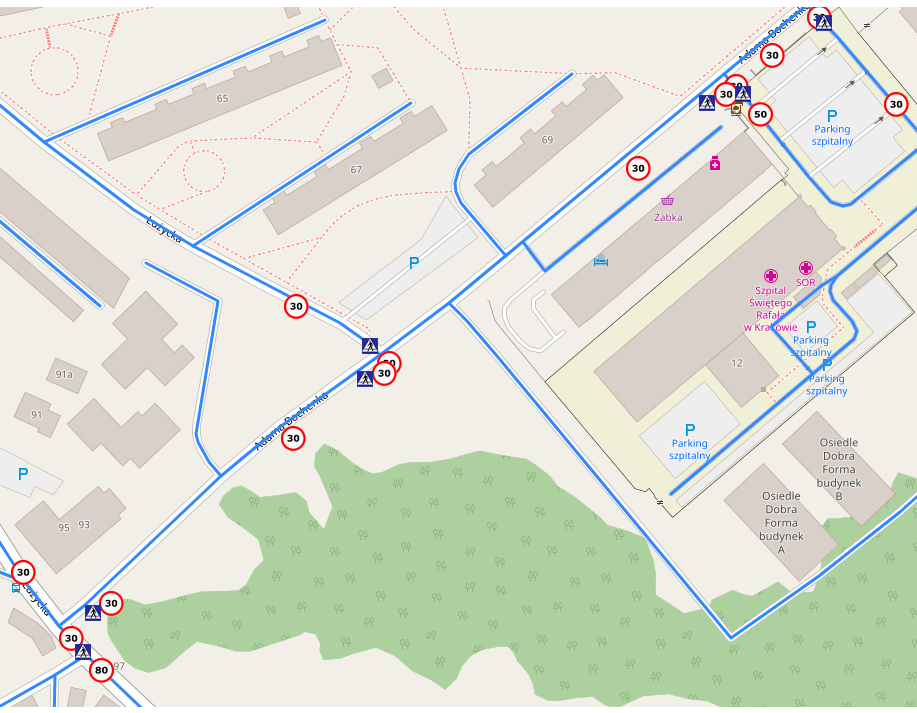
\includegraphics[width=0.9\textwidth]{pedestrian_speed}
\end{figure}

\newpage
\section{Typ nawierzchni}
\label{sec:surfaceType}

W celu zadbania o bezpieczeństwo osób, ale również o dobrą kondycję techniczną pojazdów poruszających się po drogach, niezbędne jest uwzględnienie typu nawierzchni. Nie można dopuścić do sytuacji, gdy na nawierzchni składającej się głównie że żwiru, znajdowało się znak ograniczenia prędkości o wysokiej wartości. Wtedy ulec awarii może zarówno zawieszenie, jak również pojazdy jadące przed nimi pojazdami. Aby zapoabiec tego typu problemom, podzieliłem typ nawierzchni na kilka rodzajów:

\begin{itemize}
\item kostka brukowa
\item żwir
\item drobny żwir
\item nieutwardzana
\item błotnista
\item płyty  betowowe
\item droga gruntowa
\item piasek
\item asfalt
\end{itemize}

Najbardziej problematyczna dla kierowów droga to taka, która pokryta jest żwirem, drobnym żwirem, składająca się z piasku lub jest błotnista. W takich przypadkach ograniczyłem prędkość do 10 km/h. Niewiele lepsza nawierzchnia to taka, która wyłożona jest zarówno kostką brukową oraz płytami betonowymi. Dla nich, odpowiednia prędkość wynosi 20 km/h. W przypadku drogi nieutwardzanej oraz gruntowej, ograniczenie prędkości wynosi 30 km/h. Dla asfaltu, ze względu na jego strukturę, ograniczenie prędkości praktycznie nie występuje.

Na Rys. \ref{sec:surfaceTypePhoto} zostały umieszczone ograniczenia prędkości dla dróg, których nawierzchnia pokryta jest materiałem innym niż asfalt. Dla celów demonstracyjnych, został on specjalnie pominięty, ponieważ więszkość dróg jest nim pokryta, przez co Rys. \ref{sec:surfaceTypePhoto} stałby się mało czytelny. Oczywiście ogólny algorytm uwzględnia asfalt.

\newpage
\begin{figure}[h]
\caption{Ograniczenia prędkości ze względu na rodzaj nawierzchni.}
\label{sec:surfaceTypePhoto}
\centering
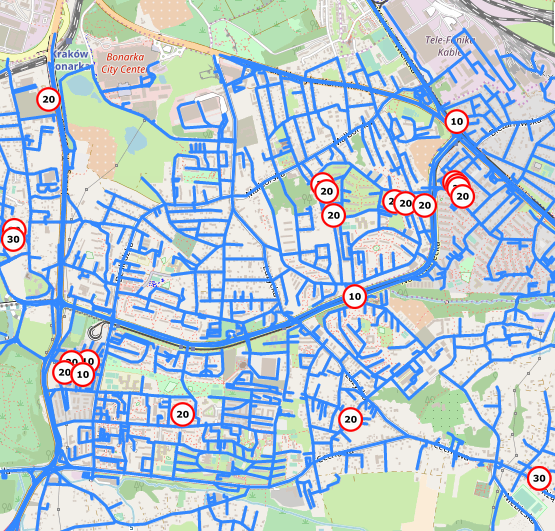
\includegraphics[width=0.9\textwidth]{surfaceType}
\end{figure}

\newpage
\section{Przejazdy kolejowe}
\subsection{Przyporządkowywanie przejazdów kolejowych do poszczególnych dróg}

Istotnych parametrem algorytmu wyznaczającego dopuszczalne prędkości jest obecność przejazdów kolejowych. Jak wiadomo, pociąg nie zatrzyma się w miejscu. Jego droga chamowania w głównej mierze zależy od masy oraz prędkości z jaką się porusza. Dla przykładu, pociąg towarowy o masie ok. 1800 ton, jadący z prędkością ok. 50 km/h, zatrzyma sie po około 500m. Dlatego ważne jest określenie prędkości, z jaką samochód moze się przemieszczać przed takim przejazdem.

Do przyporządkowania przejazdów kolejowych do poszczególnych dróg, wykorzystałem wzór \ref{eq:distancePointLineal} znajdujący się w rozdziale \ref{sec:pedestrialCrossing}


\begin{figure}[h]
\caption{Drogi na których znajdują się przejazdy kolejowe.}
\label{sec:PrzejazdyKolejowe}
\centering
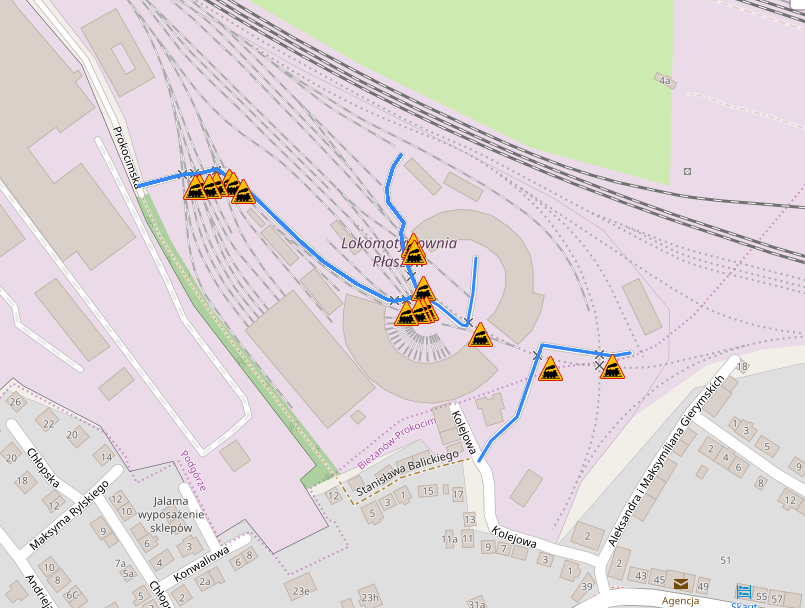
\includegraphics[width=1.0\textwidth]{railCrossing}
\end{figure}

Rys. \ref{sec:PrzejazdyKolejowe} obrazuje wynik przypisania przejazdów kolejowych do poszczególnych dróg:
\begin{itemize}
\item kolorem niebieskim drogi, na ktorych znajdują przejazdy kolejowe
\item znakiem ''A-10'' zostały oznaczone przejazdy kolejowe, pobrane z OpenStreetMap
\end{itemize}

\newpage
\subsection{Wyznaczanie prędkości i umieszczanie jej w odpowiednim miejscu na mapie}

Podobnie jak miało to miejsce w rozdziale \ref{sec:pedestrialCrossing}, umiejscowienie znaków przed przejazdem będzie zależało od kilku czynników:
\begin{itemize}
\item na  drodze z ograniczeniem prędkości do 60 km/h, znak zostanie umieszczony 50m przed przejazdem kolejowym
\item w przypadku prędkości powyżej 60 km/h, znak zostanie umieszczony w odległości 150m przed przejazdem kolejowym
\item w przypadku drogi jednokierunkowej, tylko przed przejazdem kolejowym
\item w przypadku drogi dwukierunkowej, zarówno przed, jak i za przejazdem
\item bezpośrednio za przejazdem zostanie ustawiony znak przywracającą poprzednie ograniczenie prędkości, za wyjątkiem sytuacji, gdy droga za przejazdem kolejowym jest krótsza niż 100m. W takim wypadku, nie ma sensu zmieniać prędkości.
\end{itemize}

Rys. \ref{sec:PrzejazdyKolejowe1} obrazuje przejazd kolejowy znajdujący się na dwukierunkowej drodze, na której obowiązuje ograniczenie prędkości do 80 km/h. Dlatego znaki 30 km/h zostały umieszczone 150m przed przejazdem, a zaraz po nim znaki przywracające poprzednią prędkość 80 km/h. Znaki są po obu stronach, gdyż jest do droga dwukierunkowa

\begin{figure}[h]
\caption{Umiejscowienie znaków przed i za przejazdem kolejowym.}
\label{sec:PrzejazdyKolejowe1}
\centering
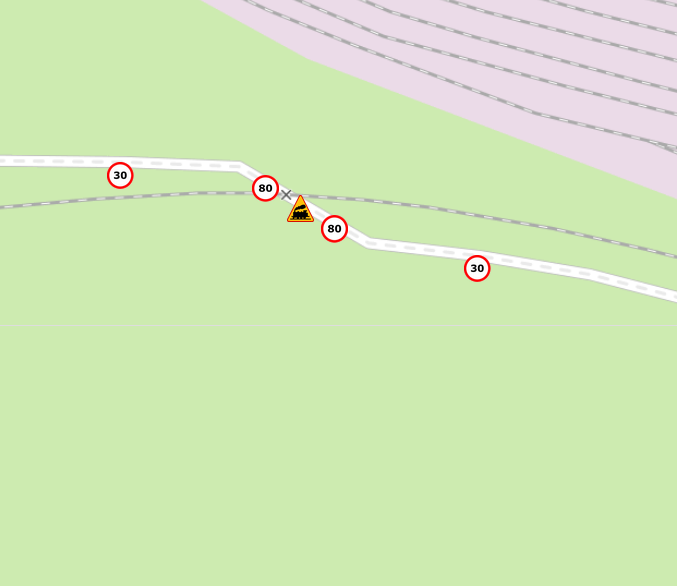
\includegraphics[width=0.7\textwidth]{streetBeforeRail}
\end{figure}


\newpage
\section{Sygnalizacja świetlna}
\subsection{Przyporządkowywanie sygnalizacji świetlnej do poszczególnych dróg}

Aby kierowca bez problemu mógł zdążyć zareagować na zmieniające się swiatło sygnalizacji świetlnej, niezbędne jest zredukowanie prędkości do odpowiedniej wartości. Ze względu na fakt iż sygnalizacja widoczna jest z relatywnie dużej odległości, prędkość przed nią zostanie ograniczona do ok. 50 km/h.


\begin{figure}[h]
\caption{Drogi na których znajduje się sygnalizacja świetlna.}
\label{sec:PrzejazdyKolejowe2}
\centering
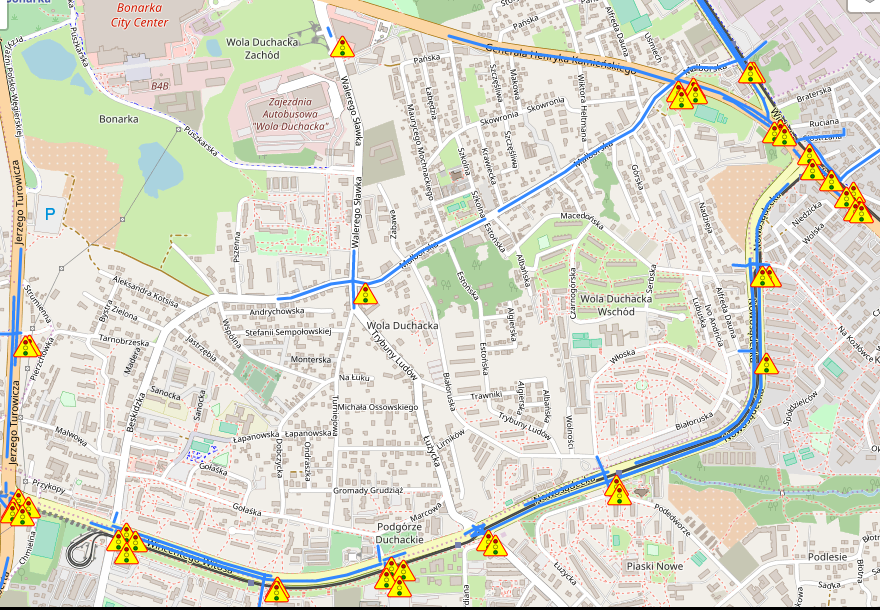
\includegraphics[width=1.1\textwidth]{traffic_sight}
\end{figure}

Rys. \ref{sec:PrzejazdyKolejowe2} ukazuje sposób działania algorytmu przypisującego do drogi sygnalizację świetlną. Zaznaczono na nim:
\begin{itemize}
\item kolorem niebieskim drogi, na ktorych znajduje się sygnalizacja świetlna
\item znakiem ''A-29'' zostały oznaczone sygnalizacje świetlne, pobrane z OpenStreetMap
\end{itemize}

\newpage
\subsection{Wyznaczanie prędkości i umieszczanie jej w odpowiednim miejscu na mapie}

Algorytm umieszcza znaki ograniczenia prędkości w następujący spasób:
\begin{itemize}
\item 50m przed sygnalizacją na drodze z ograniczeniem prędkości do 60 km/h
\item 150m przed sygnalizacją na drodze z ograniczeniem prędkości powyżej 60 km/h
\item w przypadku drogi dwukierunkowej, zarówno przed, jak i za przejazdem
\end{itemize}


Rys. \ref{sec:znakiSwiatla} obrazuje fragment skrzyżowania na której znajduje się sygnalizacja świetlna. Ograniczenie prędkości na drogach wynosi od 70 do 80 km/h, dlatego algorytm umieścił znak ograniczenia prędkości do 50 km/h, 150m przed sygnalizacją oraz znak przywracający poprzednią prędkość zaraz za sygnalizacją.

\begin{figure}[h]
\caption{Ograniczenie predkości przed i za światłami drogowymi}
\label{sec:znakiSwiatla}
\centering
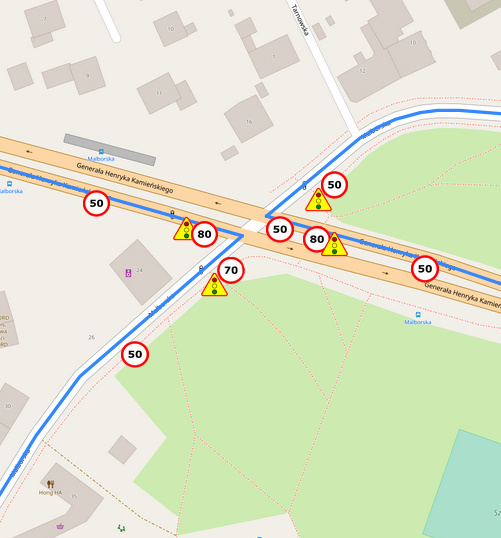
\includegraphics[width=0.8\textwidth]{speedBeforeSignals}
\end{figure}

\newpage
\section{Przystanki autobusowe i tramwajowe}


\newpage
\section{Szkoły i miesca zabaw}


\newpage
\section{Sklepy i miejsca kultów religijnych}


\newpage
\section{Liczba pasów ruchu}


\newpage
\section{Rodzaj drogi}


\newpage
\section{Płynna zmiana prędkości pojazdów}


\newpage
\section{Historia wypadków}


\newpage
\section{Zakręty}


\section{Umiejscowienie znaków na drodze}
\label{sec:speedLimitLocalization}
Znaki drogowe ograniczenia prędkości są ustawione według następujących kryteriów:
\begin{itemize}
\item na początku każdej drogi
\item przed nieoznakowanymi przejściami dla pieszych
\item przed wjazdem do obszaru, w pobliżu którego znajdują się szkoły, place zabaw, duże sklepy handlowe i miejsca kultów religijnych
\item przed zakrętami
\item między znakami ograniczenia prędkości, dla których występują duże różnice prędkości
\end{itemize}


\chapter{Algorytm - poszczególne składowe oraz przykłady zastosowania}
\label{cha:AlgorytmPraktyka}

\newpage
\section{Przejścia dla pieszych}
\label{sec:pedestrialCrossing}
\subsection{Przyporządkowywanie przejść dla pieszych do poszczególnych dróg}

Bardzo ważnym czynnikiem doboru prędkości jest obecność przejść dla pieszych. Te z sygnalizacją świetlną nie stanowią problemu, ponieważ ruch pieszych poruszających się na nich jest ograniczony tylko do sytuacji, gdy sygnalizacja świeci się na zielono. W przypadku przejść bez sygnalizacji, sprawa się komplikuje, ponieważ kierowca jest zobowiązany do zachowania szczególnej ostrożności i zmiejszenia prędkości od 30 km/h.

Do przyporządkowania przejść dla pieszych, do poszczególnych dróg, posłużyłem się wzorem \ref{eq:distancePointLineal} na odległość punktu od prostej, przedstawionym w sekcji \ref{sec:ObiektyPunktDrogi}.


Rezultatem wdrożenia powyższego wzoru do programu, są:
\begin{itemize}
\item na niebiesko zaznaczone drogi, na których znajdują się przejścia dla pieszych
\item znakiem ''D-6'' zostały oznaczone przejścia dla pieszych
\end{itemize}
Wynik został przedstawiony na Rys. \ref{sec:PrzejscieDrogi}:

\begin{figure}[h]
\caption{Drogi na których znajdują się przejścia dla pieszych.}
\label{sec:PrzejscieDrogi}
\centering
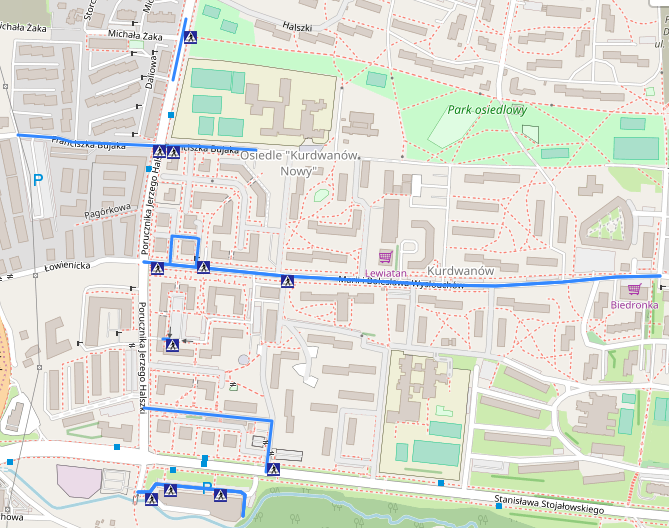
\includegraphics[width=0.9\textwidth]{PrzejscieDrogi}
\end{figure}

Dzięki tak zobrazowanej sytuacji, można ocenić skuteczność algorytmu przyporządkowującego przejścia dla pieszych do określonych dróg.

\subsection{Wyznaczanie prędkości i umieszczanie jej w odpowiednim miejscu na mapie}

Bezpieczna prędkość w pobliżu nieoznakowanych przejść dla pieszych wynosi ok. 30 km/h. Zapewnia ona zarówno wystarczajacy czas reakcji, odpowiednio krótką drogę hamowania oraz zmiejsza ryzyko wystąpień potrąceń pieszych.

Algorytm umieszcza znaki ograniczenia prędkości:
\begin{itemize}
\item w przypadku gdy maksymalna prędkość na drodze jest mniejsza bądź równo 30 km/h, nie ma sensu wstawiać znaku
\item w odległości 50 m od przejścia, gdy maksymalna prędkość na drodze jest mniejsza bądź równa 60 km/h
\item w odległości 150 m od przejścia, gdy maksymalna prędkość przekracza 60 km/h
\item w przypadku, gdy przejście dla pieszych znajduje się w odległości mniejszej niż 50m lub 150m (w zależności od maksymalnej prędkości), znak zostanie umieszczony na początku drogi
\item w przypadku drogi jednokierunkowej, tylko przed przejściem
\item w przypadku drogi dwukierunkowej, zarówno przed, jak i za przejściem
\item bezpośrednio za przejściem zostanie ustawiony znak przywracającą poprzednie ograniczenie prędkości, za wyjątkiem sytuacji, gdy droga za przejściem dla pieszych jest krótsza niż 100m. W takim wypadku, nie ma sensu zmieniać prędkości.
\end{itemize}

\begin{figure}[h]
\caption{Ograniczenia prędkości przy przejściach dla pieszych.}
\label{sec:przejsciePredkosci}
\centering
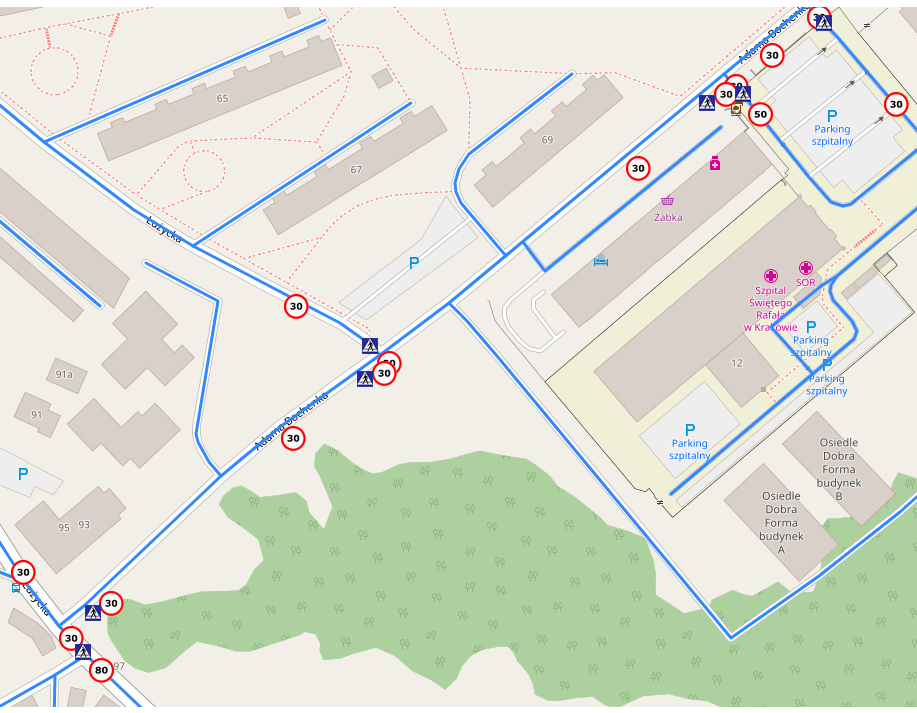
\includegraphics[width=0.7\textwidth]{pedestrian_speed}
\end{figure}

\newpage
\section{Typ nawierzchni}
\label{sec:surfaceType}

W celu zadbania o bezpieczeństwo osób, ale również o dobrą kondycję techniczną pojazdów poruszających się po drogach, niezbędne jest uwzględnienie typu nawierzchni. Nie można dopuścić do sytuacji, gdy na nawierzchni składającej się głównie że żwiru, znajdowało się znak ograniczenia prędkości o wysokiej wartości. Wtedy ulec awarii może zarówno zawieszenie, jak również pojazdy jadące przed nimi pojazdami. Aby zapoabiec tego typu problemom, podzieliłem typ nawierzchni na kilka rodzajów:

\begin{itemize}
\item kostka brukowa
\item żwir
\item drobny żwir
\item nieutwardzana
\item błotnista
\item płyty  betowowe
\item droga gruntowa
\item piasek
\item asfalt
\end{itemize}

Najbardziej problematyczna dla kierowów droga to taka, która pokryta jest żwirem, drobnym żwirem, składająca się z piasku lub jest błotnista. W takich przypadkach ograniczyłem prędkość do 10 km/h. Niewiele lepsza nawierzchnia to taka, która wyłożona jest zarówno kostką brukową oraz płytami betonowymi. Dla nich, odpowiednia prędkość wynosi 20 km/h. W przypadku drogi nieutwardzanej oraz gruntowej, ograniczenie prędkości wynosi 30 km/h. Dla asfaltu, ze względu na jego strukturę, ograniczenie prędkości praktycznie nie występuje.

Na Rys. \ref{sec:surfaceTypePhoto} zostały umieszczone ograniczenia prędkości dla dróg, których nawierzchnia pokryta jest materiałem innym niż asfalt. Dla celów demonstracyjnych, został on specjalnie pominięty, ponieważ więszkość dróg jest nim pokryta, przez co Rys. \ref{sec:surfaceTypePhoto} stałby się mało czytelny. Oczywiście ogólny algorytm uwzględnia asfalt.

\newpage
\begin{figure}[h]
\caption{Ograniczenia prędkości ze względu na rodzaj nawierzchni.}
\label{sec:surfaceTypePhoto}
\centering
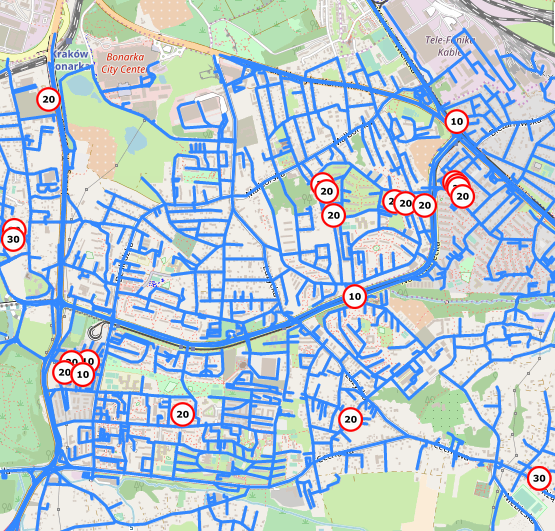
\includegraphics[width=0.9\textwidth]{surfaceType}
\end{figure}

\newpage
\section{Przejazdy kolejowe}
\subsection{Przyporządkowywanie przejazdów kolejowych do poszczególnych dróg}

Istotnych parametrem algorytmu wyznaczającego dopuszczalne prędkości jest obecność przejazdów kolejowych. Jak wiadomo, pociąg nie zatrzyma się w miejscu. Jego droga chamowania w głównej mierze zależy od masy oraz prędkości z jaką się porusza. Dla przykładu, pociąg towarowy o masie ok. 1800 ton, jadący z prędkością ok. 50 km/h, zatrzyma sie po około 500m. Dlatego ważne jest określenie prędkości, z jaką samochód moze się przemieszczać przed takim przejazdem.

Do przyporządkowania przejazdów kolejowych do poszczególnych dróg, wykorzystałem wzór \ref{eq:distancePointLineal} znajdujący się w rozdziale \ref{sec:pedestrialCrossing}


\begin{figure}[h]
\caption{Drogi na których znajdują się przejazdy kolejowe.}
\label{sec:PrzejazdyKolejowe}
\centering
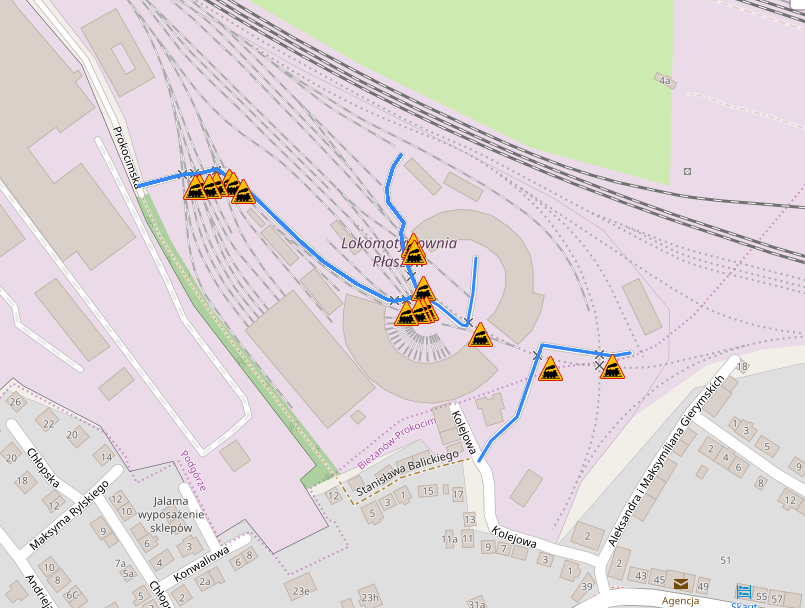
\includegraphics[width=1.0\textwidth]{railCrossing}
\end{figure}

Rys. \ref{sec:PrzejazdyKolejowe} obrazuje wynik przypisania przejazdów kolejowych do poszczególnych dróg:
\begin{itemize}
\item kolorem niebieskim drogi, na ktorych znajdują przejazdy kolejowe
\item znakiem ''A-10'' zostały oznaczone przejazdy kolejowe, pobrane z OpenStreetMap
\end{itemize}

\newpage
\subsection{Wyznaczanie prędkości i umieszczanie jej w odpowiednim miejscu na mapie}

Podobnie jak miało to miejsce w rozdziale \ref{sec:pedestrialCrossing}, umiejscowienie znaków przed przejazdem będzie zależało od kilku czynników:
\begin{itemize}
\item w przypadku gdy maksymalna prędkość na drodze jest mniejsza bądź równo 30 km/h, nie ma sensu wstawiać znaku
\item na  drodze z ograniczeniem prędkości do 60 km/h, znak zostanie umieszczony 50m przed przejazdem kolejowym
\item w przypadku prędkości powyżej 60 km/h, znak zostanie umieszczony w odległości 150m przed przejazdem kolejowym
\item w przypadku drogi jednokierunkowej, tylko przed przejazdem kolejowym
\item w przypadku drogi dwukierunkowej, zarówno przed, jak i za przejazdem
\item bezpośrednio za przejazdem zostanie ustawiony znak przywracającą poprzednie ograniczenie prędkości, za wyjątkiem sytuacji, gdy droga za przejazdem kolejowym jest krótsza niż 100m. W takim wypadku, nie ma sensu zmieniać prędkości.
\end{itemize}

Rys. \ref{sec:PrzejazdyKolejowe1} obrazuje przejazd kolejowy znajdujący się na dwukierunkowej drodze, na której obowiązuje ograniczenie prędkości do 80 km/h. Dlatego znaki 30 km/h zostały umieszczone 150m przed przejazdem, a zaraz po nim znaki przywracające poprzednią prędkość 80 km/h. Znaki są po obu stronach, gdyż jest do droga dwukierunkowa

\begin{figure}[h]
\caption{Umiejscowienie znaków przed i za przejazdem kolejowym.}
\label{sec:PrzejazdyKolejowe1}
\centering
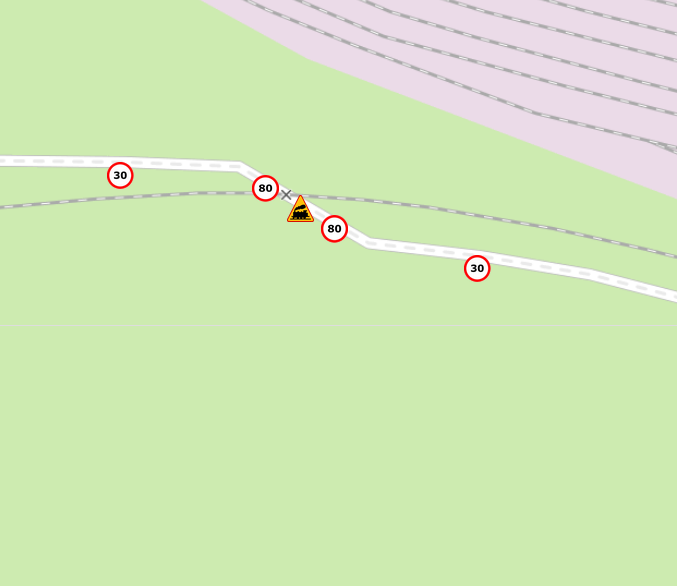
\includegraphics[width=0.6\textwidth]{streetBeforeRail}
\end{figure}


\newpage
\section{Sygnalizacja świetlna}
\subsection{Przyporządkowywanie sygnalizacji świetlnej do poszczególnych dróg}

Aby kierowca bez problemu mógł zdążyć zareagować na zmieniające się swiatło sygnalizacji świetlnej, niezbędne jest zredukowanie prędkości do odpowiedniej wartości. Ze względu na fakt iż sygnalizacja widoczna jest z relatywnie dużej odległości, prędkość przed nią zostanie ograniczona do ok. 50 km/h.


\begin{figure}[h]
\caption{Drogi na których znajduje się sygnalizacja świetlna.}
\label{sec:PrzejazdyKolejowe2}
\centering
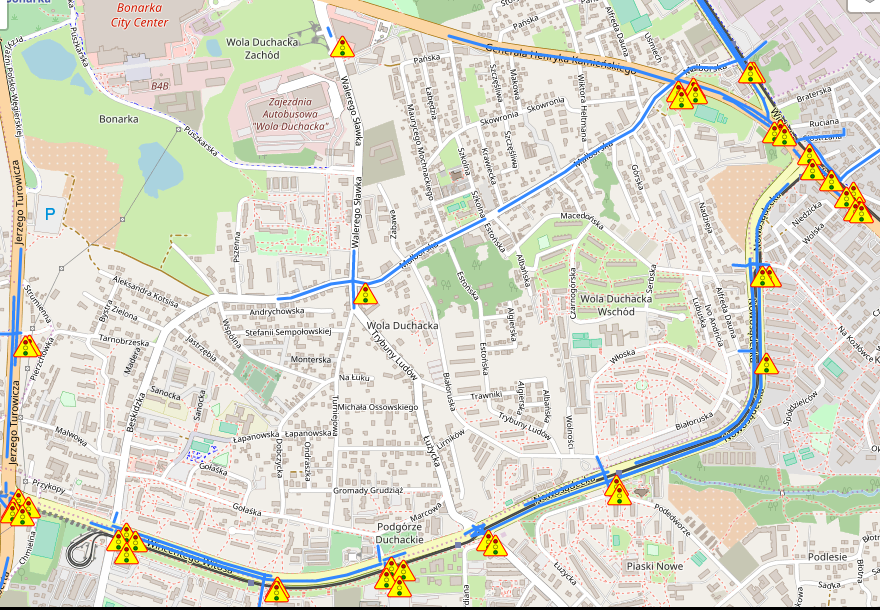
\includegraphics[width=1.1\textwidth]{traffic_sight}
\end{figure}

Rys. \ref{sec:PrzejazdyKolejowe2} ukazuje sposób działania algorytmu przypisującego do drogi sygnalizację świetlną. Zaznaczono na nim:
\begin{itemize}
\item kolorem niebieskim drogi, na ktorych znajduje się sygnalizacja świetlna
\item znakiem ''A-29'' zostały oznaczone sygnalizacje świetlne, pobrane z OpenStreetMap
\end{itemize}

\newpage
\subsection{Wyznaczanie prędkości i umieszczanie jej w odpowiednim miejscu na mapie}

Algorytm umieszcza znaki ograniczenia prędkości w następujący spasób:
\begin{itemize}
\item w przypadku gdy maksymalna prędkość na drodze jest mniejsza bądź równo 50 km/h, nie ma sensu wstawiać znaku
\item 50m przed sygnalizacją na drodze z ograniczeniem prędkości do 60 km/h
\item 150m przed sygnalizacją na drodze z ograniczeniem prędkości powyżej 60 km/h
\item w przypadku drogi dwukierunkowej, zarówno przed, jak i za przejazdem
\item bezpośrednio za przejazdem zostanie ustawiony znak przywracającą poprzednie ograniczenie prędkości, za wyjątkiem sytuacji, gdy droga za sygnalizacją świetlną jest krótsza niż 100m. W takim wypadku, nie ma sensu zmieniać prędkości.
\end{itemize}


Rys. \ref{sec:znakiSwiatla} obrazuje fragment skrzyżowania na której znajduje się sygnalizacja świetlna. Ograniczenie prędkości na drogach wynosi od 70 do 80 km/h, dlatego algorytm umieścił znak ograniczenia prędkości do 50 km/h, 150m przed sygnalizacją oraz znak przywracający poprzednią prędkość zaraz za sygnalizacją.

\begin{figure}[h]
\caption{Ograniczenie predkości przed i za światłami drogowymi}
\label{sec:znakiSwiatla}
\centering
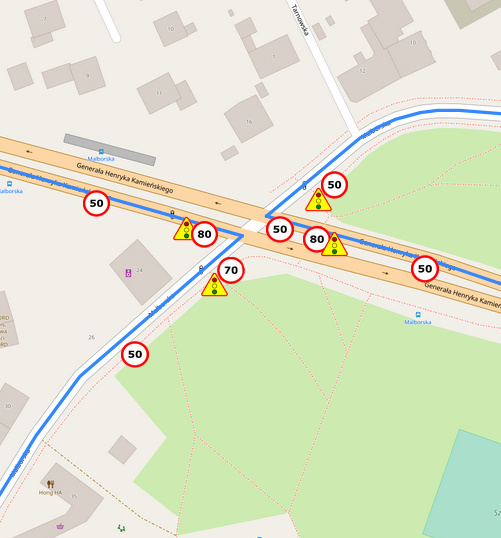
\includegraphics[width=0.6\textwidth]{speedBeforeSignals}
\end{figure}

\newpage
\section{Przystanki autobusowe i tramwajowe}
Kolejnymi obiektami, uwzględnionymi przez algorytm są przystanki autobusowe i tramwajowe. W ich pobliżu przeważnie znajduje się dość duża grupa ludzi w różnym przedziale wieku. Ponadto zdażają się sytuacje, że piesi wbiegają na drogę w celu zdążenia na komunikację miejską. Ze względu na takie zachowanie, algorytm ograniczy prędkość przy przystankach autobusowych do 30 km/h.

Na rys. \ref{sec:busStopBorder} zostały przedstawione przystanki autobusowe i tramwajowe. Wokół nich znajdują się powiększone o 5 metrów obszary pokrywający te obiekty.
\begin{figure}[h]
\caption{Ograniczenie predkości przed i za światłami drogowymi}
\label{sec:busStopBorder}
\centering
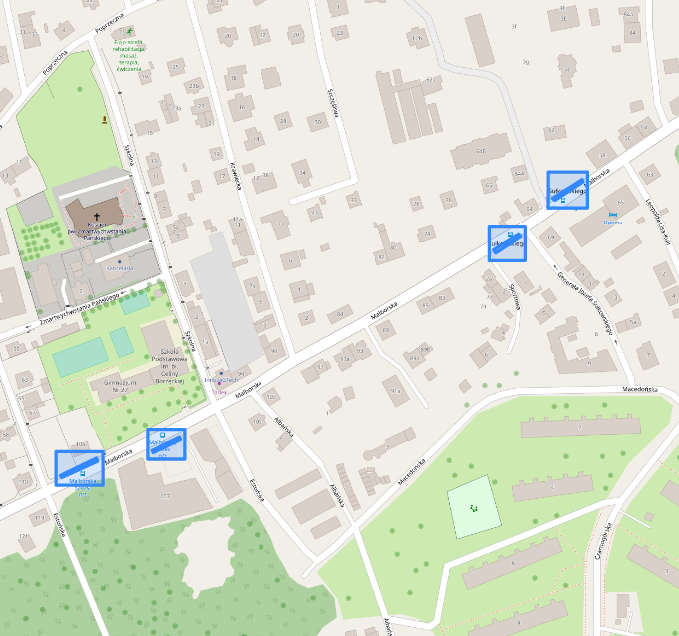
\includegraphics[width=0.9\textwidth]{busStopBorder}
\end{figure}


\newpage
\subsection{Wyznaczanie prędkości i umieszczanie jej w odpowiednim miejscu na mapie}

Najczęściej przystanki autobusowe i tramwajowe znajdują się na drogach o niezbyt wysokiej dopuszczalnej prędkości. W przypadku gdy dopuszczalna prędkość na drodze nie przekracza 30 km/h. nie ma sensu stawiać znaku. W przypadku większej prędkości znak zostanie postawiony w odległości 50 metrów od powiększonego obszaru wokół przystanku w przypadku gdy dopuszczalna prędkość nie przekracza 60 km/h. W przeciwnym razie znak zostanie postawiony w odległości 150 metrów. Znak przywracający poprzednią prędkość zaraz za nim. Opisana sytuacja została przedstawiona na rys. \ref{sec:busStopSpeed}

\begin{figure}[h]
\caption{Rozmieszczenie znaków w okolicy przystanków autobusowych}
\label{sec:busStopSpeed}
\centering
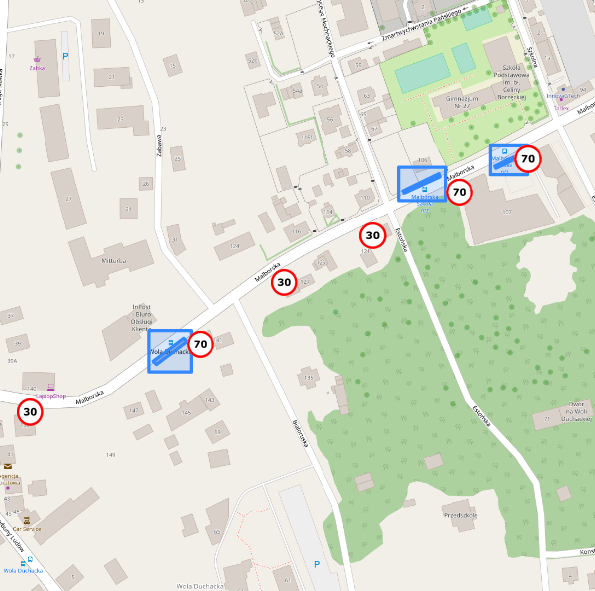
\includegraphics[width=0.9\textwidth]{busStopSpeed}
\end{figure}

\newpage
\section{Szkoły i miejsca zabaw}

Podobnie jak miało to miejsce w przypadku przystanków komunikacji miejskiej, dopuszczalna prędkość, z jaką pojazdy mogą się przenieszczać w pobliżu szkół, placów zabaw lub innych miejsc, przy których mogą znajdować się osoby niepełnoletnie, wynosi 30 km/h. Jest to niezbędne minimal, aby kierowca zdążył zareagować na czas. Rys. \ref{sec:schoolBorder} po lewej stronie przedstawia przedstawia przedszkole z placem zabaw przylegającym do niego. Natomiast po prawej znajduje się szkoła podstawowa otoczony wokół niej teren. Jak widać, zostały zaznaczone minimalnym obszarem pokrywającym, powiększonym dodatkowo o 30 metrów z każdej strony

\begin{figure}[h]
\caption{Szkoły i miejsca zabaw}
\label{sec:schoolBorder}
\centering
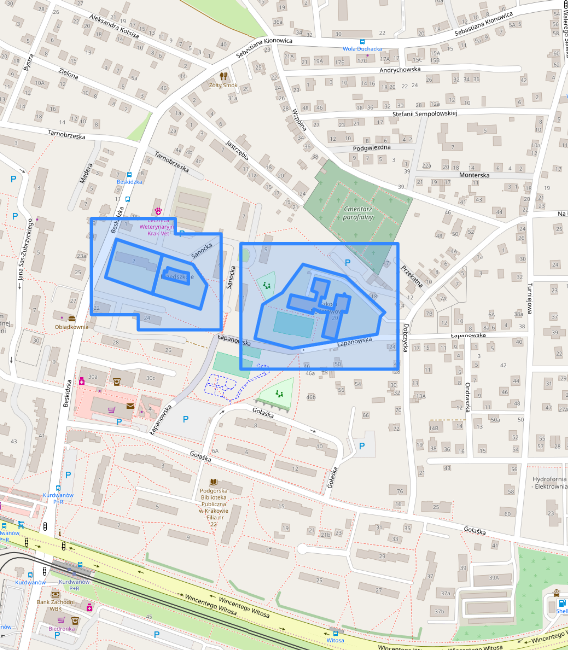
\includegraphics[width=0.9\textwidth]{schoolsBorder}
\end{figure}

\newpage
\subsection{Wyznaczanie prędkości i umieszczanie jej w odpowiednim miejscu na mapie}

Znaki ograniczające dopuszczalną prędkość zostają ustawione w odległości 50 metrów, w przypadku gdy szkoła, znajduje się w poblizu drogi z ograniczeniem prędkości do 60 km/h. Powyżej tej prędkości znaki zostają umieszczone w odległości 150m. Jest ono umieszczane tylko wtedy, gdy ograniczenie prędkości na drodze jest większe niż 30 km/h. Znak przywrocenia poprzedniego ograniczenia prędkości jest umieszczany bezpośrednio po obszarze w którym znajduje się szkoła. Zostało to przedstawione na rys. \ref{sec:schoolsSpeed}.

\begin{figure}[h]
\caption{Szkoły i miejsca zabaw}
\label{sec:schoolsSpeed}
\centering
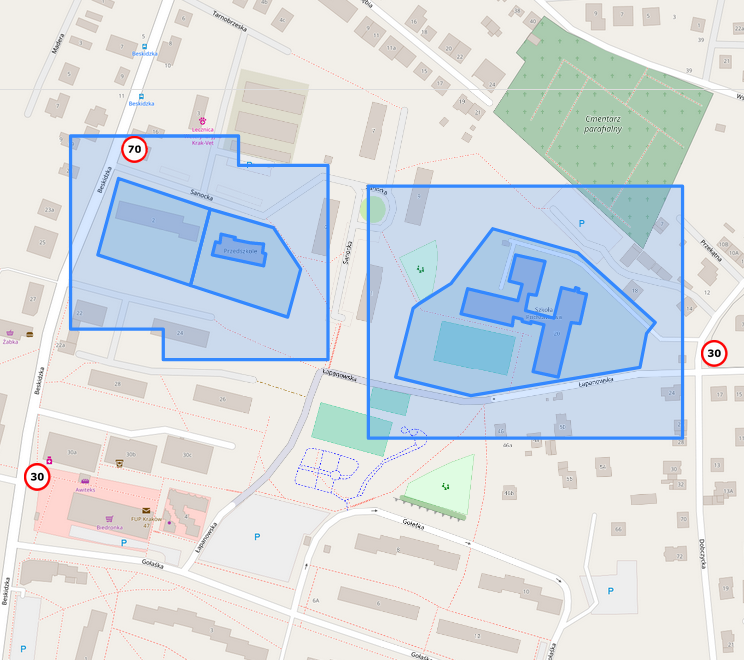
\includegraphics[width=0.95\textwidth]{schoolsSpeed}
\end{figure}

\newpage
\section{Sklepy i miejsca kultów religijnych}

\begin{figure}[h]
\caption{Szkoły i miesjca religijne}
\label{sec:shopsBorder}
\centering
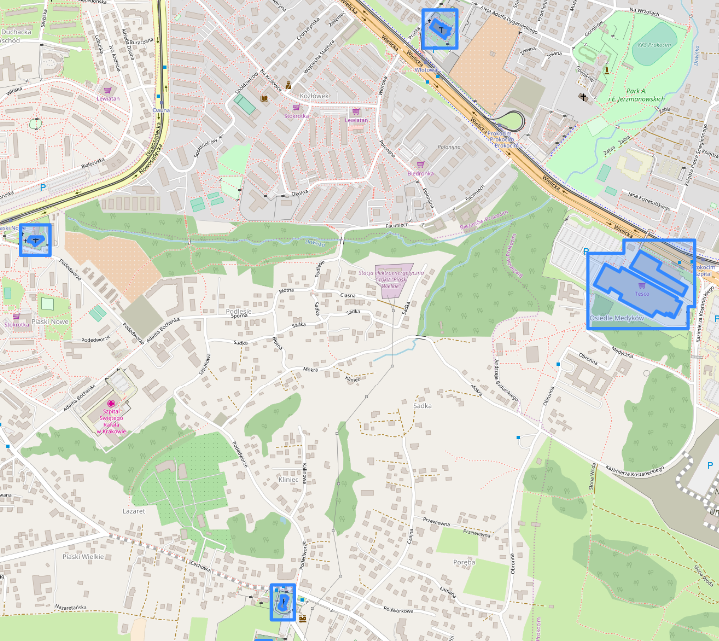
\includegraphics[width=0.9\textwidth]{shopsBorder}
\end{figure}

\newpage
\subsection{Wyznaczanie prędkości i umieszczanie jej w odpowiednim miejscu na mapie}

\begin{figure}[h]
\caption{Szkoły i miesjca religijne}
\label{sec:shopsSpeed}
\centering
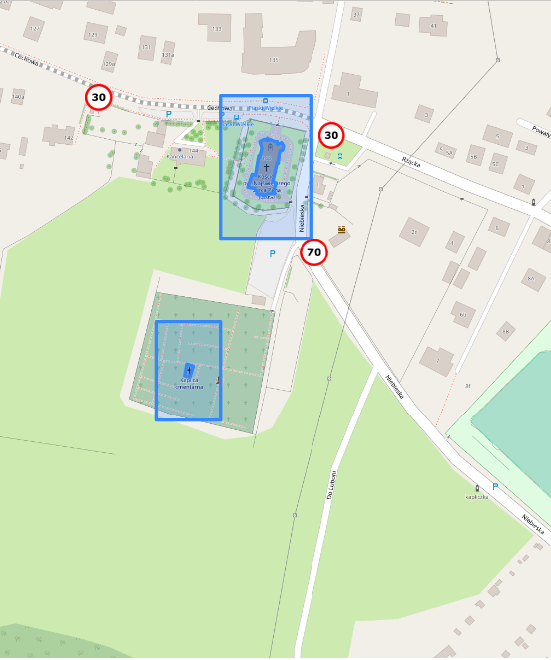
\includegraphics[width=0.9\textwidth]{shopsSpeed}
\end{figure}
\newpage
\section{Liczba pasów ruchu}

Maksymalna dozwolona prędkość jest zależna również od liczby pasów ruchu. Im jest ich więcej, tym większą prędkość można rozwijać. Dlatego algorytm zwiększa dopuszczalną prędkość o 10 km/h w przypadku gdy liczba pasów ruchu jest większa niż jeden. Na rys \ref{sec:laneNumber} zostały zaznaczone ulice, których liczba pasów ruchu wynosi przynajmniej 2, oraz prędkości nie uwzględniające pasów ruchu. 

\begin{figure}[h]
\caption{Prędkość przy nie uwgzględnieniu liczby pasów ruchu}
\label{sec:laneNumber}
\centering
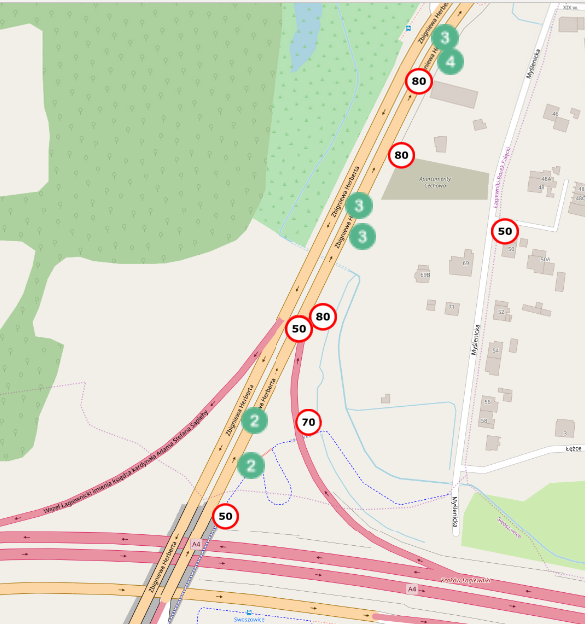
\includegraphics[width=0.9\textwidth]{laneNumber}
\end{figure}

\newpage
Na rys. \ref{sec:laneNumberAfter} zostały przedstawione prędkości już z uwzlędnioną liczbą pasów ruchu.
\begin{figure}[h]
\caption{Prędkość uwzględniająca liczbę pasów ruchu}
\label{sec:laneNumberAfter}
\centering
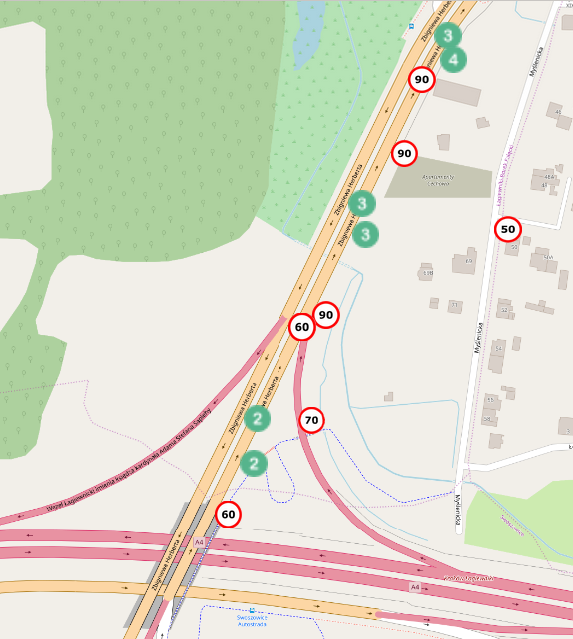
\includegraphics[width=0.9\textwidth]{laneNumberAfter}
\end{figure}

\newpage
\section{Rodzaj drogi}
Algorytm rozróżnia sześć podstawowych typów dróg, w skład których wchodzą:
\begin{itemize}
\item dojazdowe
\item lokalne
\item główne
\item główne przyspieszonego ruchu
\item ekspresowe
\item autostrady
\end{itemize}

Dla dróg dojazdowych i lokalnych ograniczenie prędkość wyznaczone przez algorytm wynosi 30 km/h. Dla dróg głównych ograniczenie prędkości wynosi 70 km/h, dla dróg głównych przyspieszonego ruchu 80 km/h, natomiast dla dróg ekspresowych 120 km/h oraz dla autostrad 140 km/h. Ograniczenia prędkości ze względu na typ drogi zostały przedstawione na rys \ref{sec:typeOfRoad}
\begin{figure}[h]
\caption{Ograniczenie prędkości w zależności od rodzajów dróg}
\label{sec:typeOfRoad}
\centering
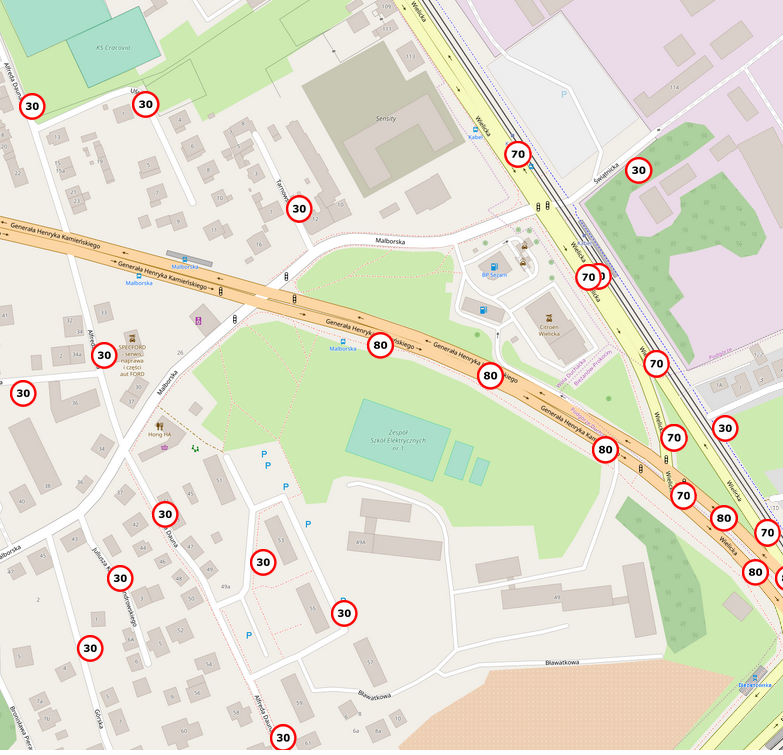
\includegraphics[width=0.7\textwidth]{typeOfRoad}
\end{figure}

\newpage
\section{Zakręty}
Ostatnim czynnikiem wpływającym na prędkość wyznaczoną przez algorytm są zakręty. Każdy zakręt posiada wyliczony swój promień skrętu. Dokładny opis ich wyznaczenia został przedstawiony w sekcji \ref{sec:WyznaczaniePromieniaSkrętuDlaZakrętówDanejDrogi}
Na rys. \ref{sec:zakrety} zostały zakręty, dla których promień skrętu jest większy niż 50m
\begin{figure}[h]
\caption{Zaznaczone zakręty}
\label{sec:zakrety}
\centering
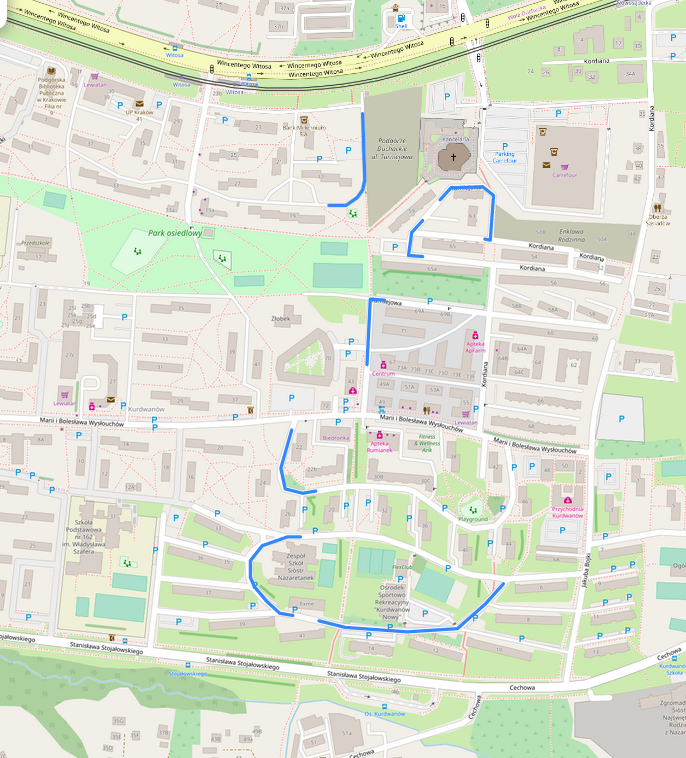
\includegraphics[width=0.9\textwidth]{zakrety}
\end{figure}

\newpage
\section{Płynna zmiana prędkości pojazdów}


\newpage
\section{Umiejscowienie znaków na drodze}
\label{sec:speedLimitLocalization}
Znaki drogowe ograniczenia prędkości są ustawione według następujących kryteriów:
\begin{itemize}
\item na początku każdej drogi
\item przed nieoznakowanymi przejściami dla pieszych
\item przed wjazdem do obszaru, w pobliżu którego znajdują się szkoły, place zabaw, duże sklepy handlowe i miejsca kultów religijnych
\item przed zakrętami
\item między znakami ograniczenia prędkości, dla których występują duże różnice prędkości
\end{itemize}



\chapter{Interfejs użytkownika}
\label{cha:UI}
Niniejszy rozdział skupia się na szczegółowym opisie interfejsu użytkownika. Zostały przedstawione najważniejsze funkcję, które pomogą użytkownikom w korzystaniu z programu. Omówiono poszczególne warstwy wyświetlone na mapie, przełączanie między nimi oraz dodawanie nowych obiektów punktowych jak również dwuwymiarowych.
W pierwszej sekcji został przedstawiony widok główny aplikacji wraz z dokładnym omówieniem. W dalszych częsciach tego rozdziału, zostały opisane kolejne warstwy. Na końcu przedstawiony został sposób, na dodawanie własnych obiektów.
\section{Widok główny aplikacji}
\label{sec:mainView}

Rys. \ref{mainView}. przedstawia widok główny aplikacji. W lewym górnym rogu znajdują się dwa przyciski: ''+'' oraz ''-''. Umożliwiają one przybliżanie i oddalanie widoku mapy. W prawym górnym rogu znajduję się menu wyboru wyświetlanej warstwy. Szczegóły dostępne w rozdziale \ref{sec:layerMenu}. Ponadto, użytkownik posiada możliwość, za pomocą myszki, przesuwania obecnie wyświetlanej mapy w dowolnym kierunku. Mapa pobierana jest w czasie rzeczywistym ze strony OpenStreetMap. Na dole znajdują się dwa nieaktywne pola typu input, służące do wyświetlania współrzędnych, jedna lista wyboru, przycisk do dodawania kolejnych współrzędnych oraz przycisk do dodawania obiektu. Lista wyboru umożliwia wybranie jednej z sześciu kategorii:
\begin{itemize}
\item \textbf{traffic signal} - sygnalizacji świetlnej
\item \textbf{pedestrian crossing} - przejcie dla pieszych
\item \textbf{rail crossing} - przejazd kolejowy
\item \textbf{bus stop} - przystanek autobusowy lub tramwajowy
\item \textbf{schools} - szkoła
\item \textbf{shops churches} - sklep lub miejce kultu religijnego
\end{itemize}

\newpage
\begin{figure}[h]
\caption{Widok główny aplikacji}
\label{mainView}
\centering
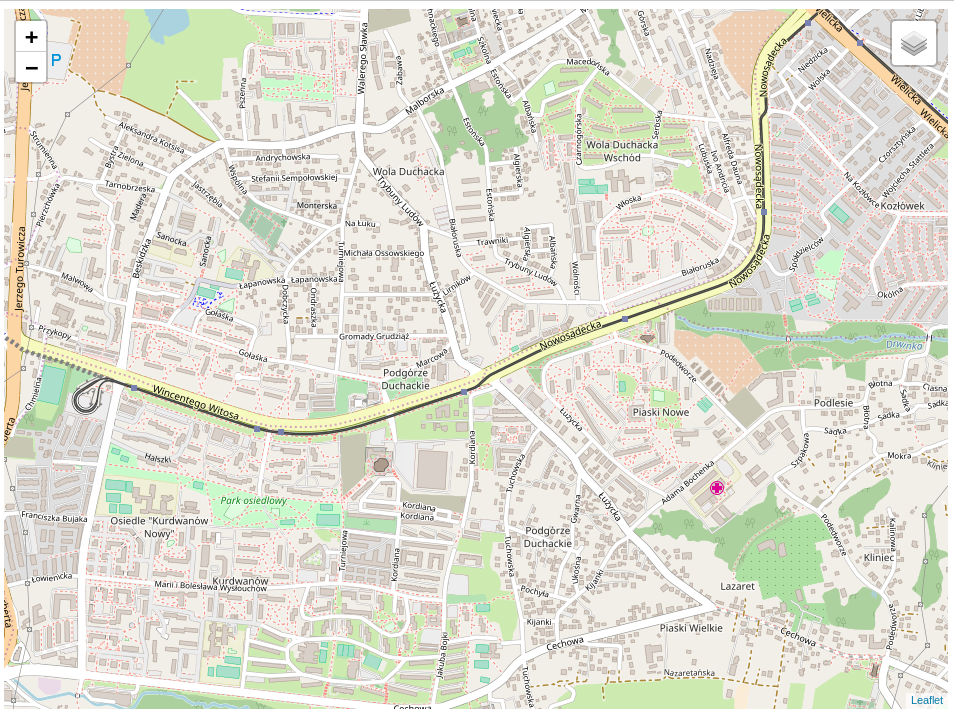
\includegraphics[width=1.02\textwidth]{mainScreen}
\end{figure}

\newpage

\section{Menu wyboru warstw}
\label{sec:layerMenu}

Rys. \ref{sec:mainLayerView}. przedstawia menu wyboru warstw. Dostępny jest dopiero po najechaniu kursorem myszy w prawy górny róg. Umozliwia wyświetlanie na mapie elementów, które użytkownik w danej chwili potrzebuje. 

\begin{figure}[h]
\caption{Menu wyboru warstw}
\label{sec:mainLayerView}
\centering
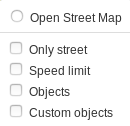
\includegraphics[width=0.55\textwidth]{layerMenu}
\end{figure}

Menu wyboru warst, Rys. \ref{sec:mainLayerView}, składa się z 35 elementów:
\begin{itemize}
\item \textbf{Only street} - służy do zaznaczania na mapie, wszystkich dostępnych ulic. Więcej szczegółów znajduje się w rozdziale \ref{sec:onlyStreet}
\item \textbf{One way streets} - zaznacza na mapie drogi jednokierunkowe
\item \textbf{pedestrian crossing, pedestrian crossing street i pedestrian crossing speed} - zaznacza na mapie odpowiednio przejścia dla pieszych, ulice na których się one znajdują oraz ograniczenia prędkości. Szczegóły zostały opisane w rozdziale \ref{sec:pedestrialCrossing} 
\item \textbf{rail crossing, rail crossing street i rail crossing speed} - zaznacza na mapie odpowiednio przejazdy kolejowe, ulice na których się one znajdują oraz ograniczenia prędkości. Szczegóły zostały opisane w rozdziale \ref{sec:railCrossingMain} 
\item \textbf{traffic signal, traffic signal street i traffic signal speed} - zaznacza na mapie odpowiednio sygnalizacje świetlną, ulice na których się one znajdują oraz ograniczenia prędkości. Szczegóły zostały opisane w rozdziale \ref{sec:trafficSignalMain} 
\item \textbf{bus stop, bus stop bounding box, bus stop street, bus stop start oraz bus stop end} - zaznacza na mapie odpowiednio przystanki autobusowe i tramwajowe, minimalny obszar pokrywający te przystanki powiększony o 5 metrów, ulice na których znajdują się przystanki, znaki początku oraz końca ograniczenia prędkości. Szczegóły opisane zostały w rozdziale \ref{sec:busStopsMain}
\item \textbf{school, school bounding box, school street, school start oraz school end} - zaznacza na mapie odpowiednio szkoły, minimalny obszar pokrywający szkoły powiększony o 30 metrów, ulice przy których znajdują się szkoły, znaki początku oraz końca ograniczenia prędkości. Szczegóły opisane zostały w rozdziale \ref{sec:schoolsMain}
\item \textbf{shops churches, shops churches bounding box, shops churches street, shops churches start oraz shops churches end} - zaznacza na mapie odpowiednio sklepy i miejsca kultów religijnych, minimalny obszar pokrywający te obiekty powiększony o 30 metrów, ulice przy których znajdują się te obiekty, znaki początku oraz końca ograniczenia prędkości. Szczegóły opisane zostały w rozdziale \ref{sec:shoopsChurchesMain}
\item \textbf{number of lanes, number of lanes speed} - zaznacza na mapie odpowiednio liczbę pasów ruchu oraz prędkość z nimi związaną. Szczegóły zostały opisane w rozdziale \ref{sec:laneNumber}
\item \textbf{type of road speed} - zaznacza na mapie ograniczenia prędkości związane z typem nawierzchni. Szczegóły zostały opisane w rozdziale \ref{sec:typeOfRoad}
\item \textbf{Curves, Curves speed start, Curves speed end} - zaznacza na mapie odpowiednio zakręty, znaki początku i końca ograniczenia prędkości dotyczące zakrętów. Szczegóły zostały opisane w rozdziale \ref{sec:zakretyMain}
\item \textbf{finished speed, finished speed street} - Najważniejsza warstwa. Umieszcza ograniczenia prędkości ma mapie, wyznaczone na podstawie wszystkich powyższych składowych. Szczegóły zostały opisane w rozdziale \ref{sec:speedLimitLocalization}
\end{itemize}

Istotną funkcjonalnością jest możliwość wyświetlania dowolnych kombinacji warstw. Użytkownik może zaznaczyć dowolną liczbę widoków, które zostaną wyswietlone na głównej mapie.

\newpage
\section{Widok zaznaczonych ulic}
\label{sec:onlyStreet}

Rys. \ref{sec:onlyStreetMap} przedstawia mapę, na której zaznaczone są poszczególne odcinki dróg. Reprezentowane są przez niebieskie linie łamane, przebiegającą przez sam jej środek. Zostały uzglednione różnego rodzaju klasy dróg, takie jak: 
\begin{itemize}
\item autostrady
\item drogi ekspresowe
\item drogi główne ruchu przyspieszonego
\item drogi główne
\item drogi zbiorcze
\item drogi lokalne
\item drogi dojazdowe
\end{itemize}

\begin{figure}[h]
\caption{Widok zaznaczonych ulic}
\label{sec:onlyStreetMap}
\centering
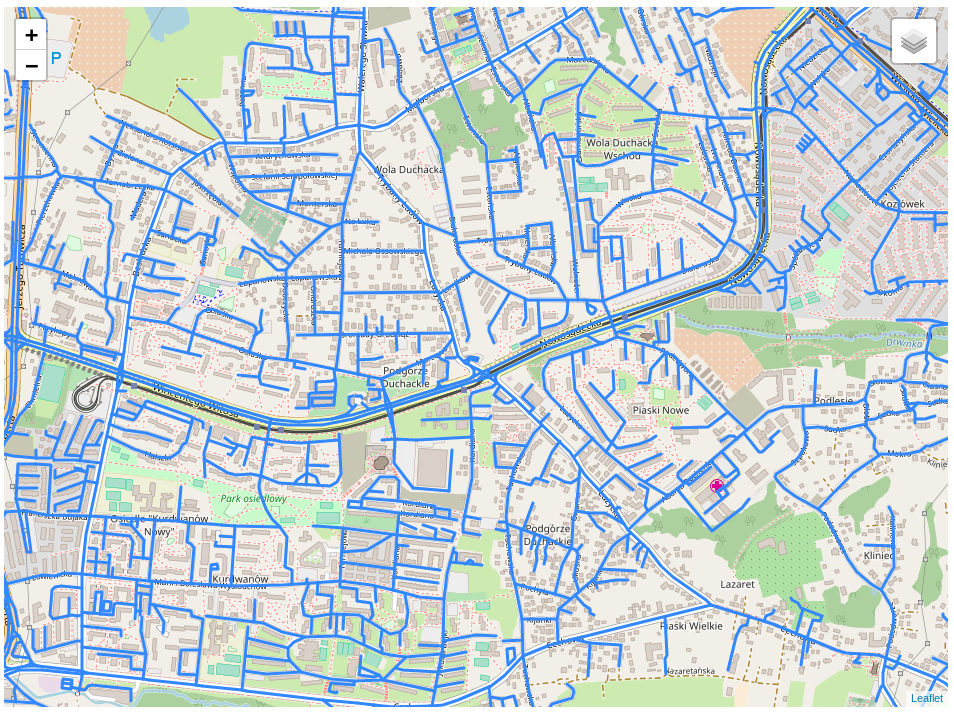
\includegraphics[width=1.03\textwidth]{onlyStreet}
\end{figure}

\newpage
\section{Dodawanie własnych obiektów}
\label{sec:addedCustomObjects}

% itd.
% \appendix
% \include{dodatekA}
% \include{dodatekB}
% itd.



\printbibliography

\end{document}
